\chapter{采用线性误差模型的可伸缩视频码流截取方案}

能够调整数据源的码率是流媒体系统码率自适应的前提条件。对于SVC视频而言,这意味着从整个码流中截取出一部分数据包。如何在给定的码率下使得截取的失真最小,是码流截取问题的关键。在本章中,我们提出一个线性误差模型和一个基于贪心思想的优先级赋值算法来解决这个问题。

\section{线性误差模型}

\subsection{模型推导}

在H.264/AVC中,解码过程具有线性性质\supercite{Winken2008}。在不考虑舍入、截断和去块滤波的情况下,解码的主要步骤,如预测、变换、量化等,都可以近似认为是线性操作。基于此,整个解码过程可以用矩阵的形式描述如下:

\begin{equation}
\label{eq:linear}
s = {\rm\bf M} \cdot s + {\rm\bf T} \cdot c + p \: .
\end{equation}

该式子意味着,一个图像组(GOP)的重建像素, $s$,可以看作如下这三部分的线性组合:该图像组的已重建像素、残差、静态预测子。在公式(\ref{eq:linear})中,$c$指代变换系数,$p$是所谓静态预测子;$\rm\bf M$和$\rm\bf T$都是方阵,${\rm\bf M} \cdot s$得到的结果是运动校正预测信号,${\rm\bf T} \cdot c$得到的结果是残差。$\rm\bf M$的实际值由所选择的宏块类型、参考帧索引和运动向量决定,而$\rm\bf T$的实际值取决于所选的量化参数(QP)。

将上述线性解码模型运用到SVC的质量可伸缩中,可以得到一个线性误差模型(LEM)。根据公式(\ref{eq:linear}),对于一个只包含基本层的码流,有:
\begin{equation}
\label{eq:base0}
s_{B} = {\rm\bf M} \cdot s_{B} + {\rm\bf T}_{B} \cdot c_{B} + p \: ,
\end{equation}
其中带下标$B$的表示是基本层变量。在质量可伸缩中,增强层主要是变换系数的精细化。因此,若一个增强层的数据包集合记为$I_1$,则含有该增强层的码流解码时重建关系可表示为:
\begin{equation}
\label{eq:subset1}
s_{I_1} = {\rm\bf M} \cdot s_{I_1} + {\rm\bf T}_{B} \cdot c_{B} + \Big( \sum_{i \in I_1}{\rm\bf T}_i \cdot c_i \Big) + p \: ,
\end{equation}
其中$i$表示集合$I_1$中的一个增强数据包;$c_i$是一个向量,含有增强层数据包$i$中的变换系数;${\rm\bf T}_i$是由$i$的QP值所决定的变换矩阵,而${\rm\bf T}_i \cdot c_i$得到的就是从$i$解码出来的残差值。

同样的,对于一个含有增强层数据包集合$I_2$的码流,有:
\begin{equation}
\label{eq:subset2}
s_{I_2} = {\rm\bf M} \cdot s_{I_2} + {\rm\bf T}_{B} \cdot c_{B} + \Big( \sum_{i \in I_2}{\rm\bf T}_i \cdot c_i \Big) + p \: .
\end{equation}

\begin{figure}[t]
	\centering
	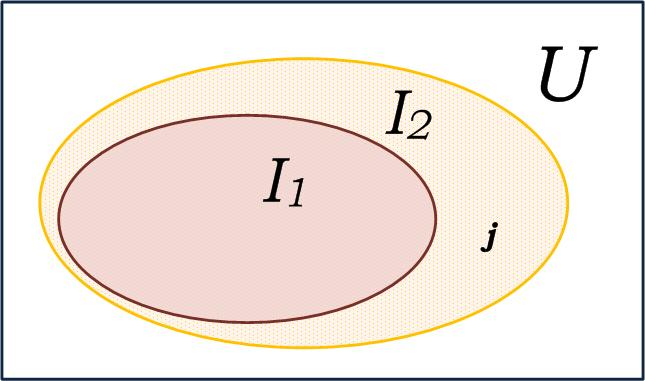
\includegraphics[width = 0.5\linewidth]{figures/Subset.jpg}
	\caption{增强层数据包集合关系示例 \label{fig:subset}}
\end{figure}

如果$I_1$是$I_2$的子集,那么二者的重建误差就可以由公式(\ref{eq:subset2})与(\ref{eq:subset1})相减得到:
\begin{equation}
\label{eq:minus1}
(s_{I_2} - s_{I_1}) = {\rm\bf M} \cdot (s_{I_2} - s_{I_1}) + \Big( \sum_{i \in I_2}{\rm\bf T}_i \cdot c_i - \sum_{i \in I_1}{\rm\bf T}_i \cdot c_i \Big) \: ,
\end{equation}
\begin{equation}
\label{eq:minus2}
\Rightarrow e = s_{I_2} - s_{I_1} = ({\rm\bf I - M})^{-1} \cdot \Big( \sum_{i \in I_2}{\rm\bf T}_i \cdot c_i - \sum_{i \in I_1}{\rm\bf T}_i \cdot c_i \Big) \: .
\end{equation}

特别地,如果$I_2$和$I_1$的差别只有一个增强层数据包$j$,也就是说$I_2 \setminus I_1 = \{j\}$(如图\ref{fig:subset}所示),那么根据公式(\ref{eq:minus2}),这两个重建序列的差为:
\begin{equation}
\label{eq:error_j}
e_j = ({\rm\bf I - M})^{-1} \cdot {\rm\bf T}_j \cdot c_j \: .
\end{equation}

可以看到,$e_j$只由数据包$j$决定,与其他的增强层数据包无关。这个值$e_j$被定义为数据包$j$的“误差向量”,表示丢弃数据包$j$后所带来的像素值误差。我们可以通过如下的方式得到任何一个数据包$j$的误差向量:选取两个只差$j$的数据包子集,将它们解码得到的视频序列相减即可。

一旦获取了所有增强层数据包对应的误差向量,那么丢弃任意一个增强层数据包子集所导致的失真就可以用这个子集中的数据包的误差向量之和来估计。举例来说,如果增强层数据包$x$, $y$, $z$从一个码流中被丢弃,那么丢弃前后的重建序列之差应该为:
\begin{equation}
e = e_x + e_y + e_z.
\end{equation}
这个简单的相加之所以合理有两方面的原因。第一,不像MSE或PSNR,误差向量仅仅是像素的差值,并不涉及二次方运算。第二,每个增强层数据包在重建中会各自对像素进行精细化,其效果是叠加的(参见前面的推导过程)。

应该指出,上述第二点原因的成立是有条件的。在公式(\ref{eq:base0})到(\ref{eq:subset2})中,${\rm\bf M}$和$p$的值都相同是因为,在质量可伸缩的情况下,增强层数据包仅仅是通过操作变换系数得到的,并不涉及运动校正和静态预测过程。然而这对于其他维度的可伸缩(例如视频分辨率改变的空间可伸缩)并不正确。因此,此处推导的线性误差模型并不适用于任意配置的可伸缩视频编码。在本文的研究中,只用到了质量可伸缩;其他伸缩维度将作为未来工作中的探索对象。

\subsection{误差向量获取}

如果按照上一小节中所说,每次计算一个数据包的误差向量,那么所需的解码次数将是所有数据包的个数。这么做的计算量太大。在本小节中,我们给出一个高效获取所有误差向量的方法。

\begin{figure}[h]
\centering
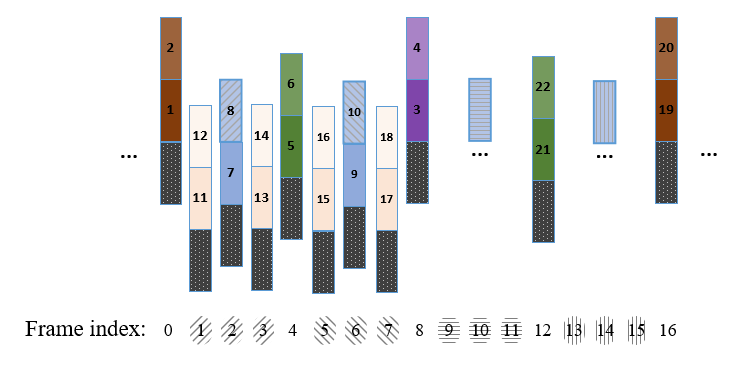
\includegraphics[width = 0.9\linewidth]{figures/GOP-Structure.png}
\caption{SVC码流中的图像组(GOP)结构示例 \label{fig:GOP_Structure}}
\end{figure}

为了减少解码次数,我们将所有的增强层数据包分成若干组,使得每一组中的多个误差向量能在一次解码中同时获取。考虑如图\ref{fig:GOP_Structure}所示具有8帧图像组结构的一个视频码流。在该图中,基本层数据包是黑色的,增强层数据包按照颜色分为了几个组(相同颜色的属于同一组)。在每一组中,增强层数据包的误差向量可以同时计算,因为这些数据包所影响的像素是互不干扰的。例如,丢弃8号数据包只会在帧1、2、3中带来像素误差,而丢弃10号数据包只会在帧5、6、7中带来像素误差(帧的编号从0开始)。因此,我们可以只通过一次相减来同时得到8号和10号数据包的误差向量$e_{8}$和$e_{10}$,以及所有其他GOP中的相同位置数据包(用相同颜色表示它们属于同一组)的误差向量。应该指出,这些误差向量是非常稀疏的,因为丢弃单个数据包带来的失真影响非常有限。

为了获取所有的误差向量,所需的解码次数大约等于增强层的层数$(L_Q - 1)$乘以时间层的层数$L_T$。对于图\ref{fig:GOP_Structure}中的例子而言,$L_Q = 3$,$L_T = 4$,所以所需的解码次数照此计算将会是$(3 - 1) \times 4 = 8$。然而,我们还需要额外的$L_Q - 1 = 2$次解码,来分离“关键帧”\supercite{H.264-Overview}(图\ref{fig:GOP_Structure}中的帧0、8、16)中数据包的失真影响。关键帧中增强层数据包的丢弃将会给它两边相邻的两个GOP都带来失真。例如,丢弃4号数据包带来的失真影响范围将会从帧1直到帧15,从而与帧0和帧16中的数据包的失真影响互相交叠。因此,关键帧同一位置的增强层数据包(2、4、20号数据包)应该被分为两个组:一组包含偶数GOP的关键帧数据包(2和20号包),另一组包含奇数GOP的(4号包)。于是,误差向量获取真正所需要的解码次数应为:
\begin{equation}
N = (L_Q - 1) \cdot (L_T + 1).
\end{equation}
这与JSVM中Quality Layer信息的获取所需的解码次数大致相当。

\subsection{失真估计与模型验证}
\label{subsec:distortion-estimation}

基于线性误差模型,我们可以估计丢弃任意增强层数据包组合带来的失真,只需把所丢弃的每一个数据包对应的误差向量加起来即可。

例如,对于一个通过丢弃数据包集合$I_x$而得到的子流来说,它解码出来的视频序列与原始序列间的差值可以估计为:
\begin{equation}
\label{eq:subset_error}
e(I_x) = e_{full} + \sum_{i \in {I_x}} e_i \: .
\end{equation}
这个公式中$e_{full}$表示全部增强层数据包都参与解码得到的视频序列与原始序列之间的差值。这是编解码过程固有的失真,在一个数据包都不丢弃的时候也是存在的。

在采用基于线性误差模型的失真估计之前,我们先做实验验证一下其准确性。该实验中的码流都是用JSVM编码器压缩得到的,编码采用了如图\ref{fig:GOP_Structure}所示的GOP结构,熵编码过程配置的是CABAC。每个码流基本层和增强层的QP分别为33和27。增强层通过配置Medium Grain Scalability (MGS)向量进一步划分为了2个MGS层,分别包含4个和12个变换系数。我们从码流中随机丢弃一组数据包,将得到的子流解码,然后比较实际的失真与通过线性误差模型估计的失真。解码用的是JSVM解码器,其他计算都通过MATLAB进行。对于序列{\em Foreman}的一个比较结果可参见图\ref{fig:model_verification}(为简单起见,只采用了前33帧)。图中的横轴代表帧序号,纵轴表示以MSE度量的失真。实线代表真实计算的失真,虚线代表用所提出的线性误差模型估计的失真。可以看到两条线非常接近,验证了用提出的模型做失真估计的准确性。我们对所有8个SVC标准序列都进行了实验,定量计算了估计误差,如表\ref{tab:estimation-error}所示。可以看到,平均估计误差只有5\%,进一步说明了模型的准确性。

\begin{figure}[h]
	\centering
	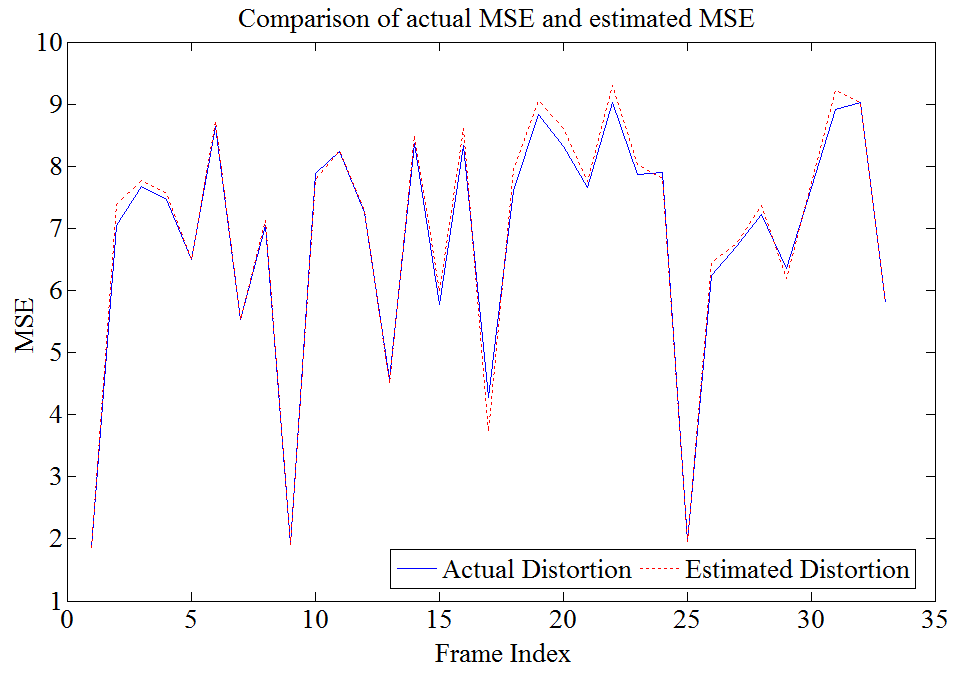
\includegraphics[width = 0.8\linewidth]{figures/ModelVerification.png}
	\caption{{\em Foreman}序列估计失真与实际失真的比较 \label{fig:model_verification}}
\end{figure}

\begin{table}[h]
	\centering
	\caption{采用线性误差模型进行不同序列失真估计的估计误差}
	\label{tab:estimation-error}
	\begin{tabular}{*{8}{p{1.35cm}<{\centering}|}{p{1.3cm}<{\centering}}}
		\hline\hline
		{\em Bus} & {\em City} & {\em Crew} & {\em Football} & {\em Foreman} & {\em Harbour} & {\em Mobile} & {\em Soccer} & \textbf{Average} \\ \hline
		2.83\% & 2.39\% & 10.36\% & 7.08\% & 4.95\% & 2.63\% & 5.77\% & 5.26\% & \textbf{5.16\%} \\ \hline
	\end{tabular}
\end{table}

\section{码流截取方案}
\label{extraction}

在这一节中,我们采用上面提出的线性误差模型来进行码流截取。因为找到码流截取问题的最优解不太现实,我们的方案采用贪心法\footnote{https://en.wikipedia.org/wiki/Greedy\_algorithm}来获得一个次优解。与“0-1背包问题”的贪心解法类似,每次当一个数据包需要被丢弃时,我们选择具有最小的码率失真影响的包。一个包的码率失真影响可以被认为决定它是否重要的优先级度量标准。下面我们首先对所采用的这个度量标准做简单的介绍,然后具体给出优先级赋值的算法。

\subsection{数据包优先级度量}

对于一个数据包,我们采用如下的码率失真影响来度量它的优先级:
\begin{equation}
\label{eq:rd_impact}
\Phi = \dfrac{\partial D}{\partial R} \: ,
\end{equation}
其中$\partial D$表示丢弃这个数据包所带来的失真的变化,而$\partial R$是相应的码率的变化。$\partial R$显然只与该数据包本身的大小有关,很容易得到。但$\partial D$的真实值需要通过分别计算丢包前后的失真来求取,在码流截取中只能估计。

这一度量标准具有直观上的意义。如果丢弃了一个数据包之后所带来的码率变化很小($\partial R$小),而丢掉它产生的失真变化却很大($\partial D$大),那意味着这个数据包非常重要,其优先级高($\Phi$大),在码流截取中应该尽量予以保留。这样的数据包本身没有很多数据,但它所处的帧被较多的其他帧所参考,丢弃之后具有较大的失真影响。采用公式(\ref{eq:rd_impact})所示的度量标准能够全面考虑到这种情形。

\subsection{优先级赋值的贪心算法}
\label{subsec:priority-assign}

我们将模拟依次从一个码流中丢掉所有增强层数据包的过程,丢包顺序就按照上面所说的贪心策略。这个顺序就作为数据包的优先级值被记录下来。这些优先级值可以被存储在码流中(NALU头信息的优先级ID字段或者补充增强信息SEI中),用于实际的码流截取。本节详细介绍优先级赋值的算法。

对于很长的视频序列,往往将其分为一个个优化窗口进行操作。每个窗口含有一定数量的帧,优先级赋值和码流截取都在每个窗口中独立地进行。假设优化窗口的长度为$K$,也就是说每次处理$K$帧;再假设每一帧包含的质量伸缩层个数为$L_Q$,也就是一个基本层加$L_Q-1$个增强层。这样的话所有能够被丢弃的增强层数据包的个数将是$K \cdot (L_Q-1)$。在每一次贪心选择的步骤中,当前可以被丢弃的数据包只能是每一帧最上层的数据包(因为下层的包被上层所依赖),也就是最多有$K$个。在这样的优化窗口中进行优先级赋值的过程具体描述如下:

\begin{description}
	\item[1)] 初始状态下,把整个序列的误差向量$e_{seq}$设为$e_{full}$(所有增强层数据包都在时解码出的序列与原始序列的差值,参见公式(\ref{eq:subset_error})的说明)。
	\item[2)] 在所有当前可以丢弃的数据包中,找到对序列具有最小码率失真影响的数据包$m$,即寻找$m$,使得:
	\begin{equation}
	\label{eq:R-D_impact_m}
	\Phi_m = \min_{i \in I_{top}} \Phi_i \: ,
	\end{equation}
	其中$I_{top}$代表当前处于每一帧最上层的数据包,现在只有它们是可以丢弃的。一个包的失真影响基于公式(\ref{eq:rd_impact})计算如下: 
	\begin{equation}
	\label{eq:R-D_impact_i}
	\Phi_i = \dfrac{\partial D}{\partial R} = \dfrac{PSNR(e_{seq}) - PSNR(e_{seq} + e_i)}{SIZE(i)} \: ,
	\end{equation}
	其中$SIZE(i)$是数据包$i$的大小,$PSNR(*)$是由误差向量求取PSNR的函数。PSNR是由MSE定义的,而MSE就是误差向量的元素平方后的均值。
	\item[3)]将数据包$m$从码流中移除,并把它的误差向量加到序列误差向量中:
	\begin{equation}
	\label{eq:error_update}
	e_{seq} = e_{seq} + e_m \: .
	\end{equation}
	\item[4)]重复2)到3)的步骤,直到所有的增强层数据包全部被移除,且每个包都根据它被移除的次序被赋予了优先级值。
\end{description}

上面描述的过程用算法伪码表示可参见下面的Algorithm\ref{algo:greedy}。

\begin{algorithm}
	\caption{优先级赋值的贪心算法}
	\label{algo:greedy}
	\begin{algorithmic}
		\STATE 初始化$e_{seq}$为$e_{full}$, 初始化$q$为0;
		\WHILE{$q < K \cdot (L_Q - 1)$}
		\FOR{(最多)$K$个处于每帧最上层的数据包}
		\STATE 找到具有最小失真影响$\Phi_m$的数据包$m$;
		\ENDFOR
		\STATE 设置$m$的优先级为$q$;
		\STATE 将$m$从码流中移除;
		\STATE 将$e_{seq}$更新为$e_{seq} + e_m$,并将$q$更新为$q+1$;
		\ENDWHILE
	\end{algorithmic}
\end{algorithm}

从伪码很容易看出优先级赋值算法的时间复杂度为$O(K^2)$。需要指出的是,在优先级赋值过程中的这些计算量相比于误差向量获取过程中解码的计算量来说是微不足道的。通过增加优化窗口大小$K$,可以每次比较更多的数据包来确定优先级,因此有望得到更优的截取结果。然而,这样做不仅增加计算量,更重要的是会使存储误差向量所需的内存有显著的增加。此外,如果优先级值采用NALU头信息中的字段存储的话,因为该字段只有6个比特,所支持的范围是0~63,这也限制了$K$的大小。

\subsection{无参考源的情况}
\label{subsec:noref}

在某些场合,优先级赋值和码流截取需要在没有原始视频序列的情况下进行。这将增加问题的难度,因为当原始序列未知的时候更难以获取实际失真。这种无参考的情形在实际中甚至比有参考的情形更常见。因为通常来说,流媒体服务提供商拿到的都是压缩后的码流,很少能拿到原始视频序列。在这一小节中,我们对所提出的算法稍作修改以适应这种没有参考源的特殊情况。

在缺少原始序列的情况下,我们无法计算上面提到的$e_{full}$。一个简单直接的想法是把$e_{full}$置为0,也就是所有失真都是基于整个码流完全重建的像素来计算,而不是基于原始序列。但我们发现这样做效果并不好,算法过程中的PSNR值太大,无法很好的反映实际失真。这是因为丢弃一些数据包后,与完全重建像素比较起来并不能带来很大的误差,据此计算PSNR是不合适的。为了解决这个问题,我们改为直接用所有像素的均方差(MSE)作为失真的度量标准,不再计算PSNR。即,公式(\ref{eq:R-D_impact_i})应修改为:
\begin{equation}
\label{eq:R-D_impact_i_noref}
\Phi_i = \dfrac{\partial D}{\partial R} = \dfrac{MSE(e_{seq}) - MSE(e_{seq} + e_i)}{SIZE(i)} \: ,
\end{equation}
其中,$MSE(*)$表示直接由误差向量得到MSE。这样做使得无参考情况下的截取效果有所提升,被证明是一个合理有效的改进(参见下一节中的相应实验结果)。

\subsection{优先级值的实际使用}

上面所述的算法为可伸缩视频码流中的每个增强层数据包赋予了一个优先级值,这些优先级值将用于实际的码流截取。本小结具体介绍在实际系统中如何使用优先级值来进行码流截取。

首先,系统应该提前确定每个优先级值与码率的对应关系,这只需要进行一次性的统计操作。有了这个对应关系之后,在给定的截取码率下,就知道了应保留的数据包优先级下限。假设这个下限为P,则在传输时,所有增强层数据包优先级低于P的都应该丢弃。在发送一个数据包前,传输程序首先检查它是基本层数据包还是增强层数据包。如果是前者,则发送;如果是后者,则读取其优先级值与P比较。如果大于等于P,则发送;如果小于P,则将其丢弃。

在我们所实现的支持可伸缩视频的达尔文流媒体服务器中,传输时每次发送的是一个RTP包,而一个RTP包中可能包含多个或者不到一个SVC数据包,即NALU(参见\ref{subsec:protocols}小节)。考虑到这一点,服务器程序应该按照如图\ref{fig:extraction-flow}所示的流程来实现发送前的码流截取。

\begin{figure}[!ht]
	\centering
	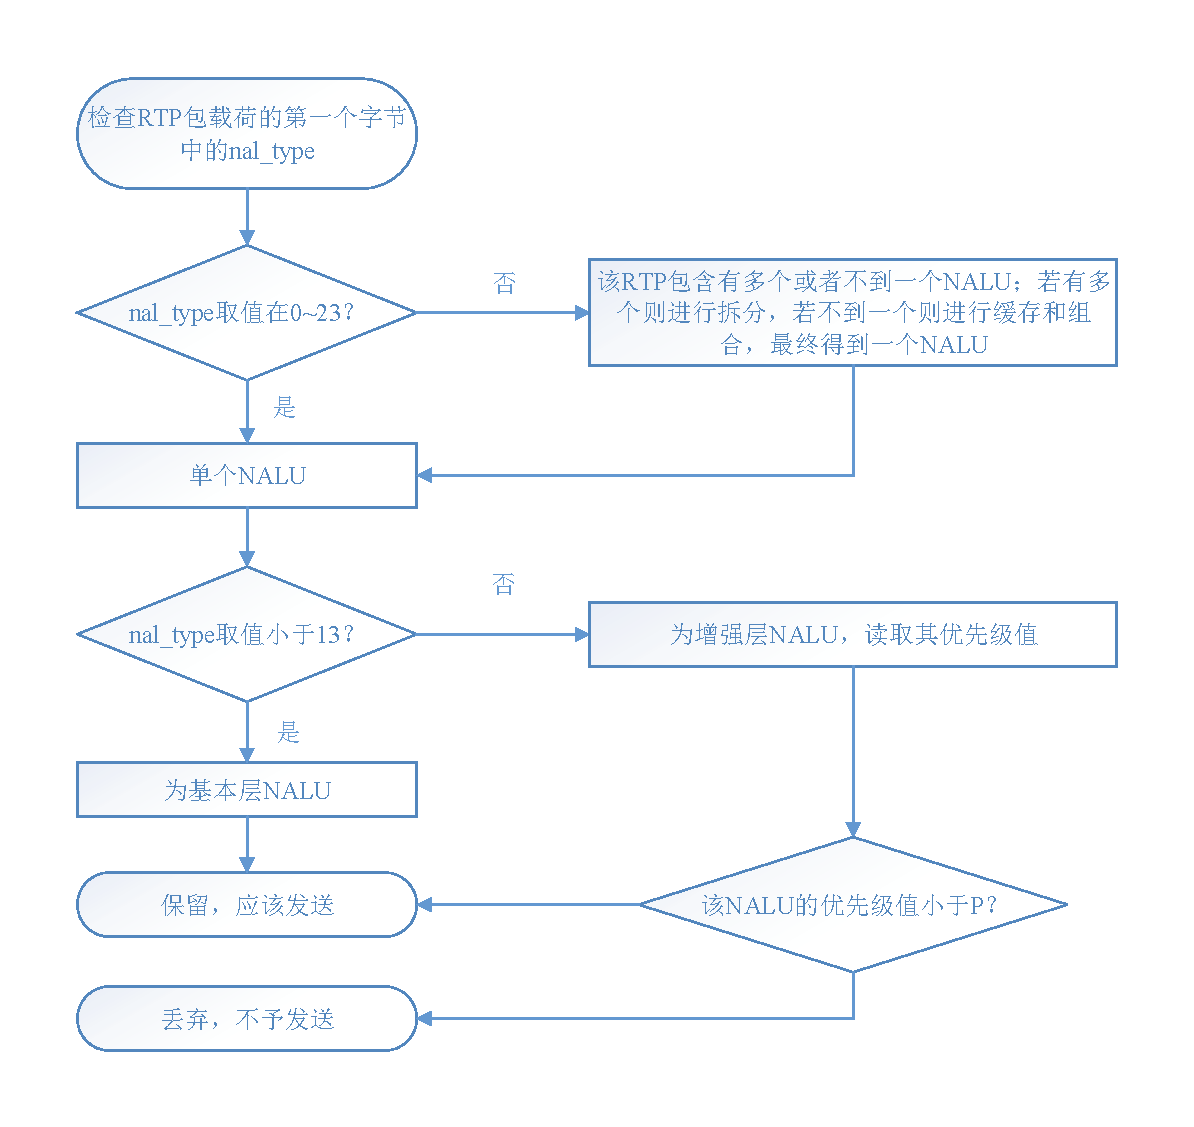
\includegraphics[width = 1.0\linewidth]{eps/extraction-flow}
	\caption{使用优先级值进行实际码流截取的程序流程图\label{fig:extraction-flow}}
\end{figure}

\section{实验结果}

本节通过与参考软件JSVM(9.16版本)的对比来展示所提出的码流截取方案的实验结果。

\subsection{实验配置}

所有的测试码流都是按照\ref{subsec:distortion-estimation}中模型验证时所述的配置编码得到的。对于每个码流,我们选取十个截取点:一个是包含所有增强层数据包的完整码流,一个是只含有基本层数据包的最低码率码流,二者之间又等距离地选取了8个码率点。对每个码率点,我们用三种方法进行截取:JSVM中的基本截取器(用JSVM Basic指代),JSVM中采用了Quality Layers的截取器(用JSVM QL指代),以及本文提出的截取器。在本文提出的截取方案中,优先级赋值算法里的优化窗口大小是32帧,也就是4个GOP(GOP大小是8)。所有CIF大小的SVC标准测试序列都进行了测试,码率计算时采用了30FPS的帧率。

\subsection{结果分析}

\begin{figure*}[!ht]
	\centering
	\subfloat[Bus]{
		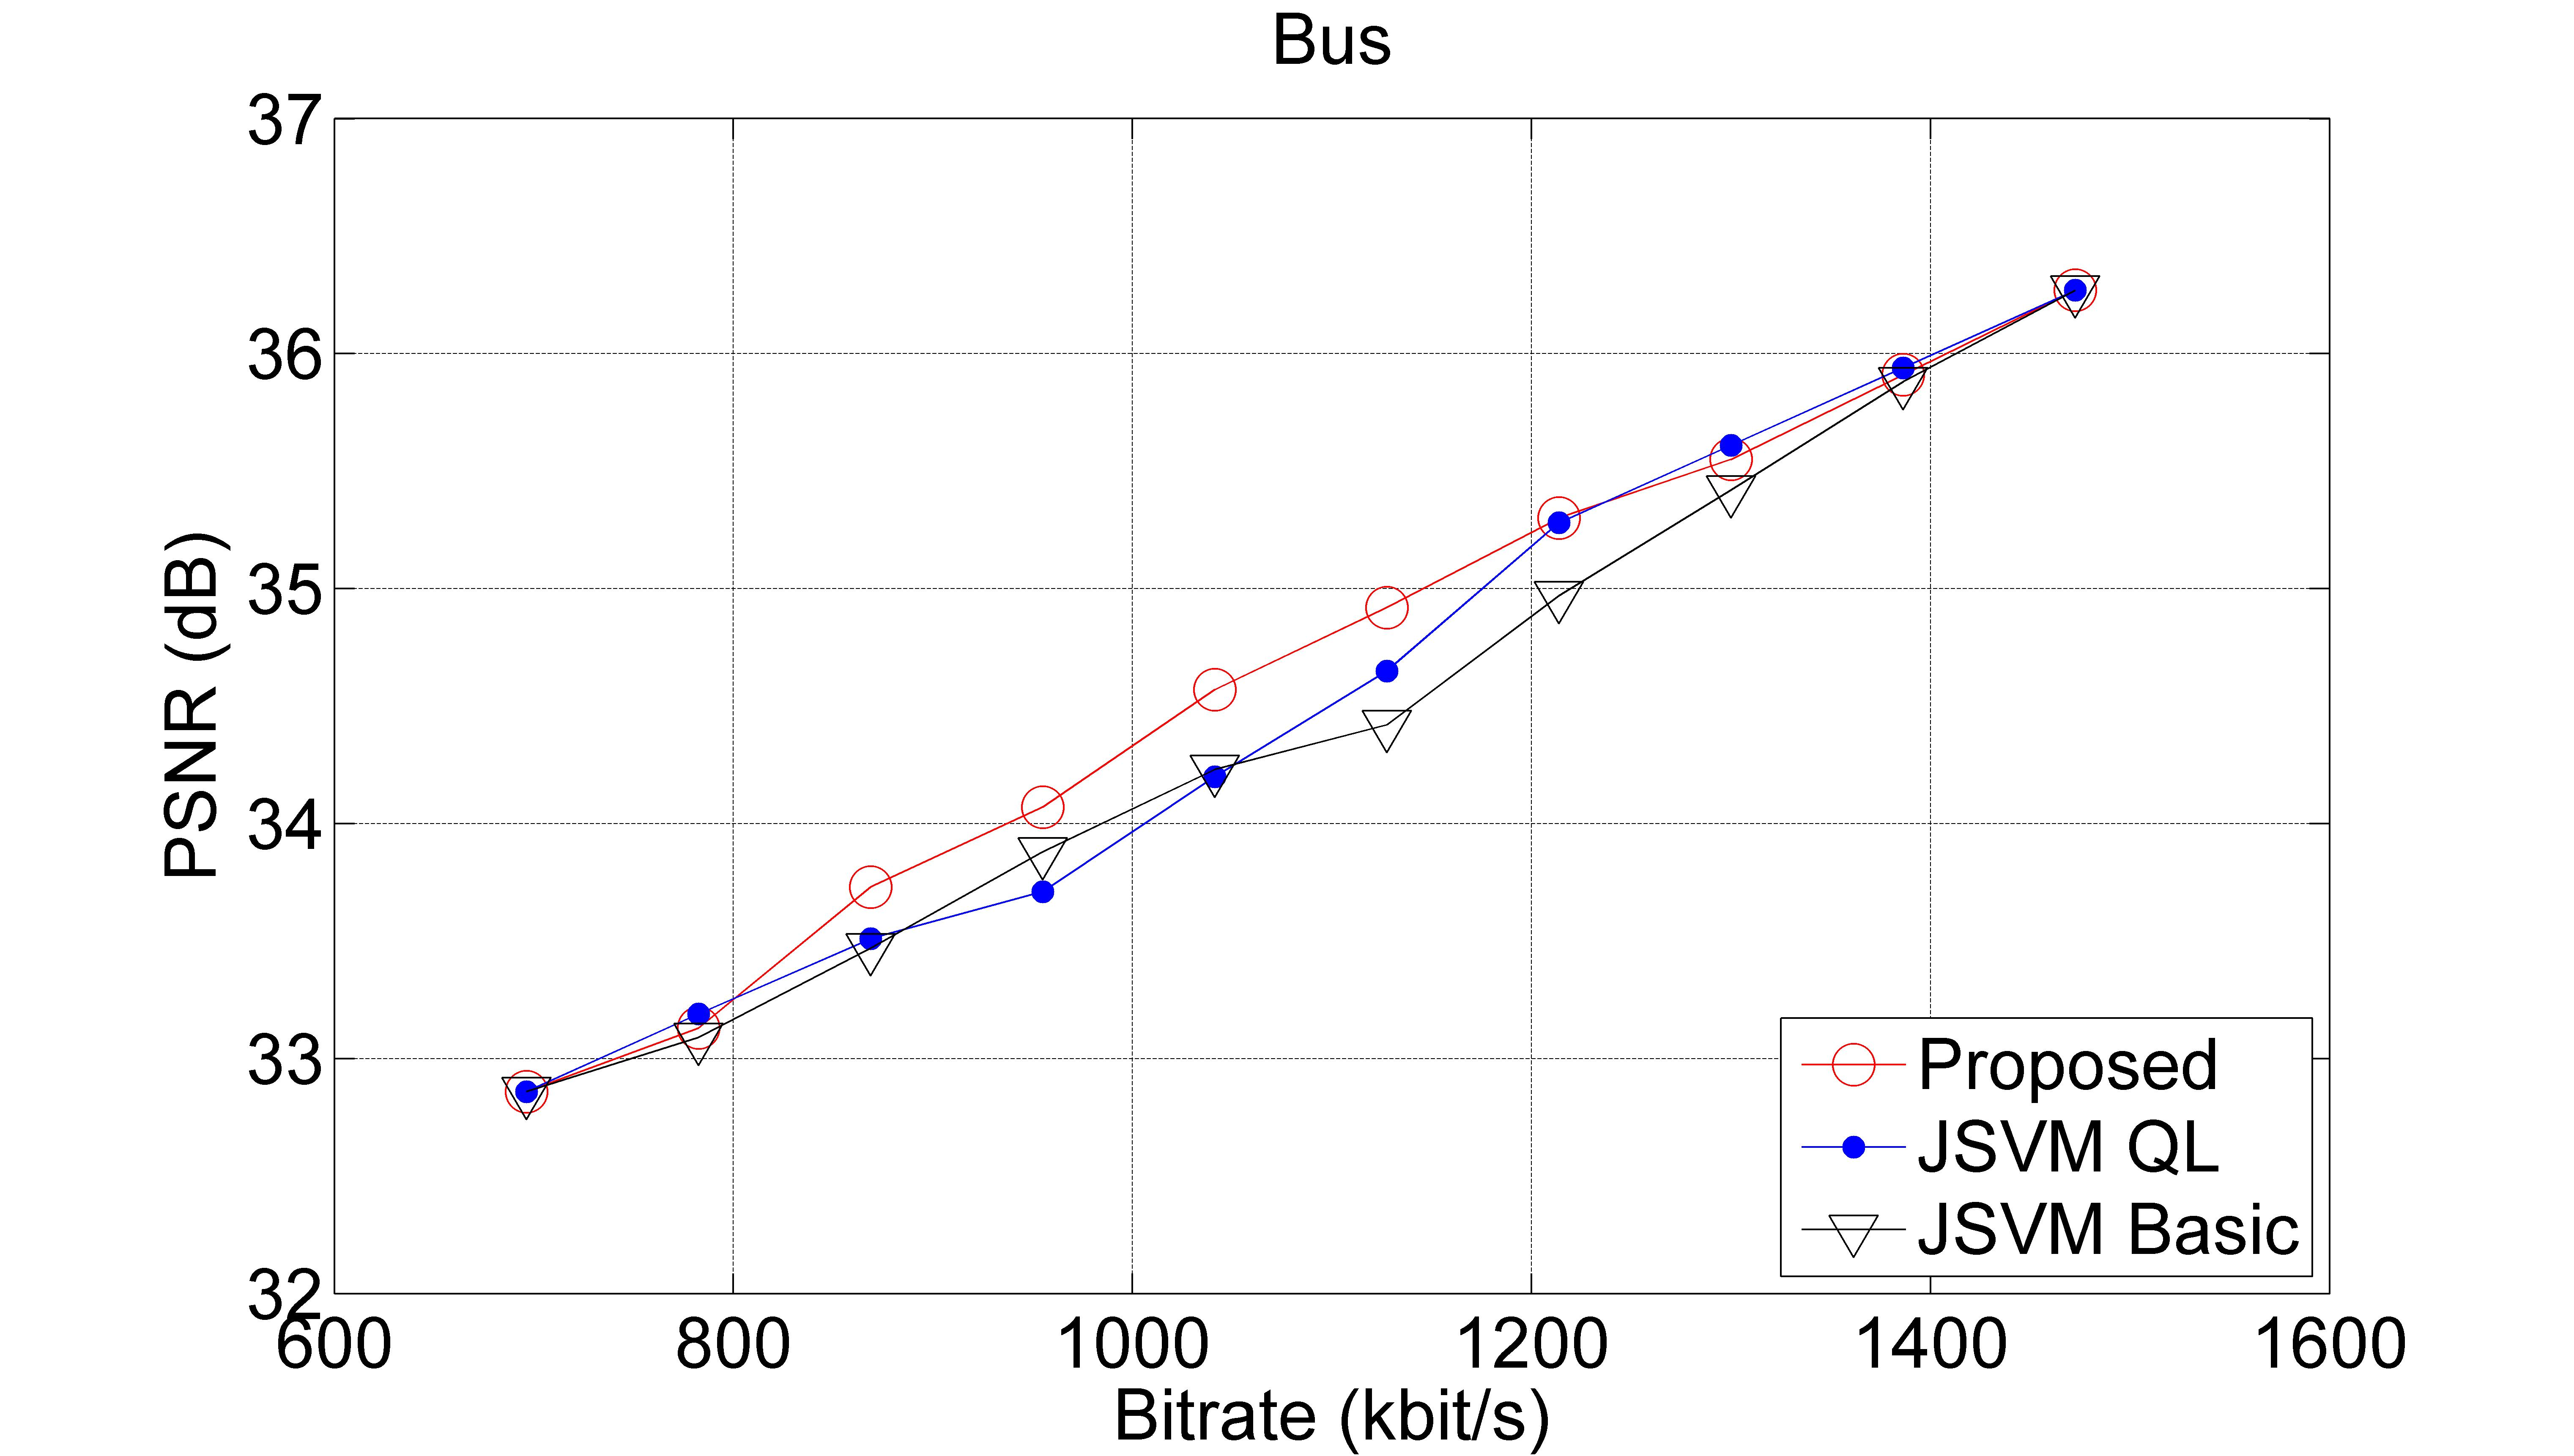
\includegraphics[width=0.5\textwidth]{figures/Bus.jpg}
		\label{fig:Bus}}
	\subfloat[City]{
		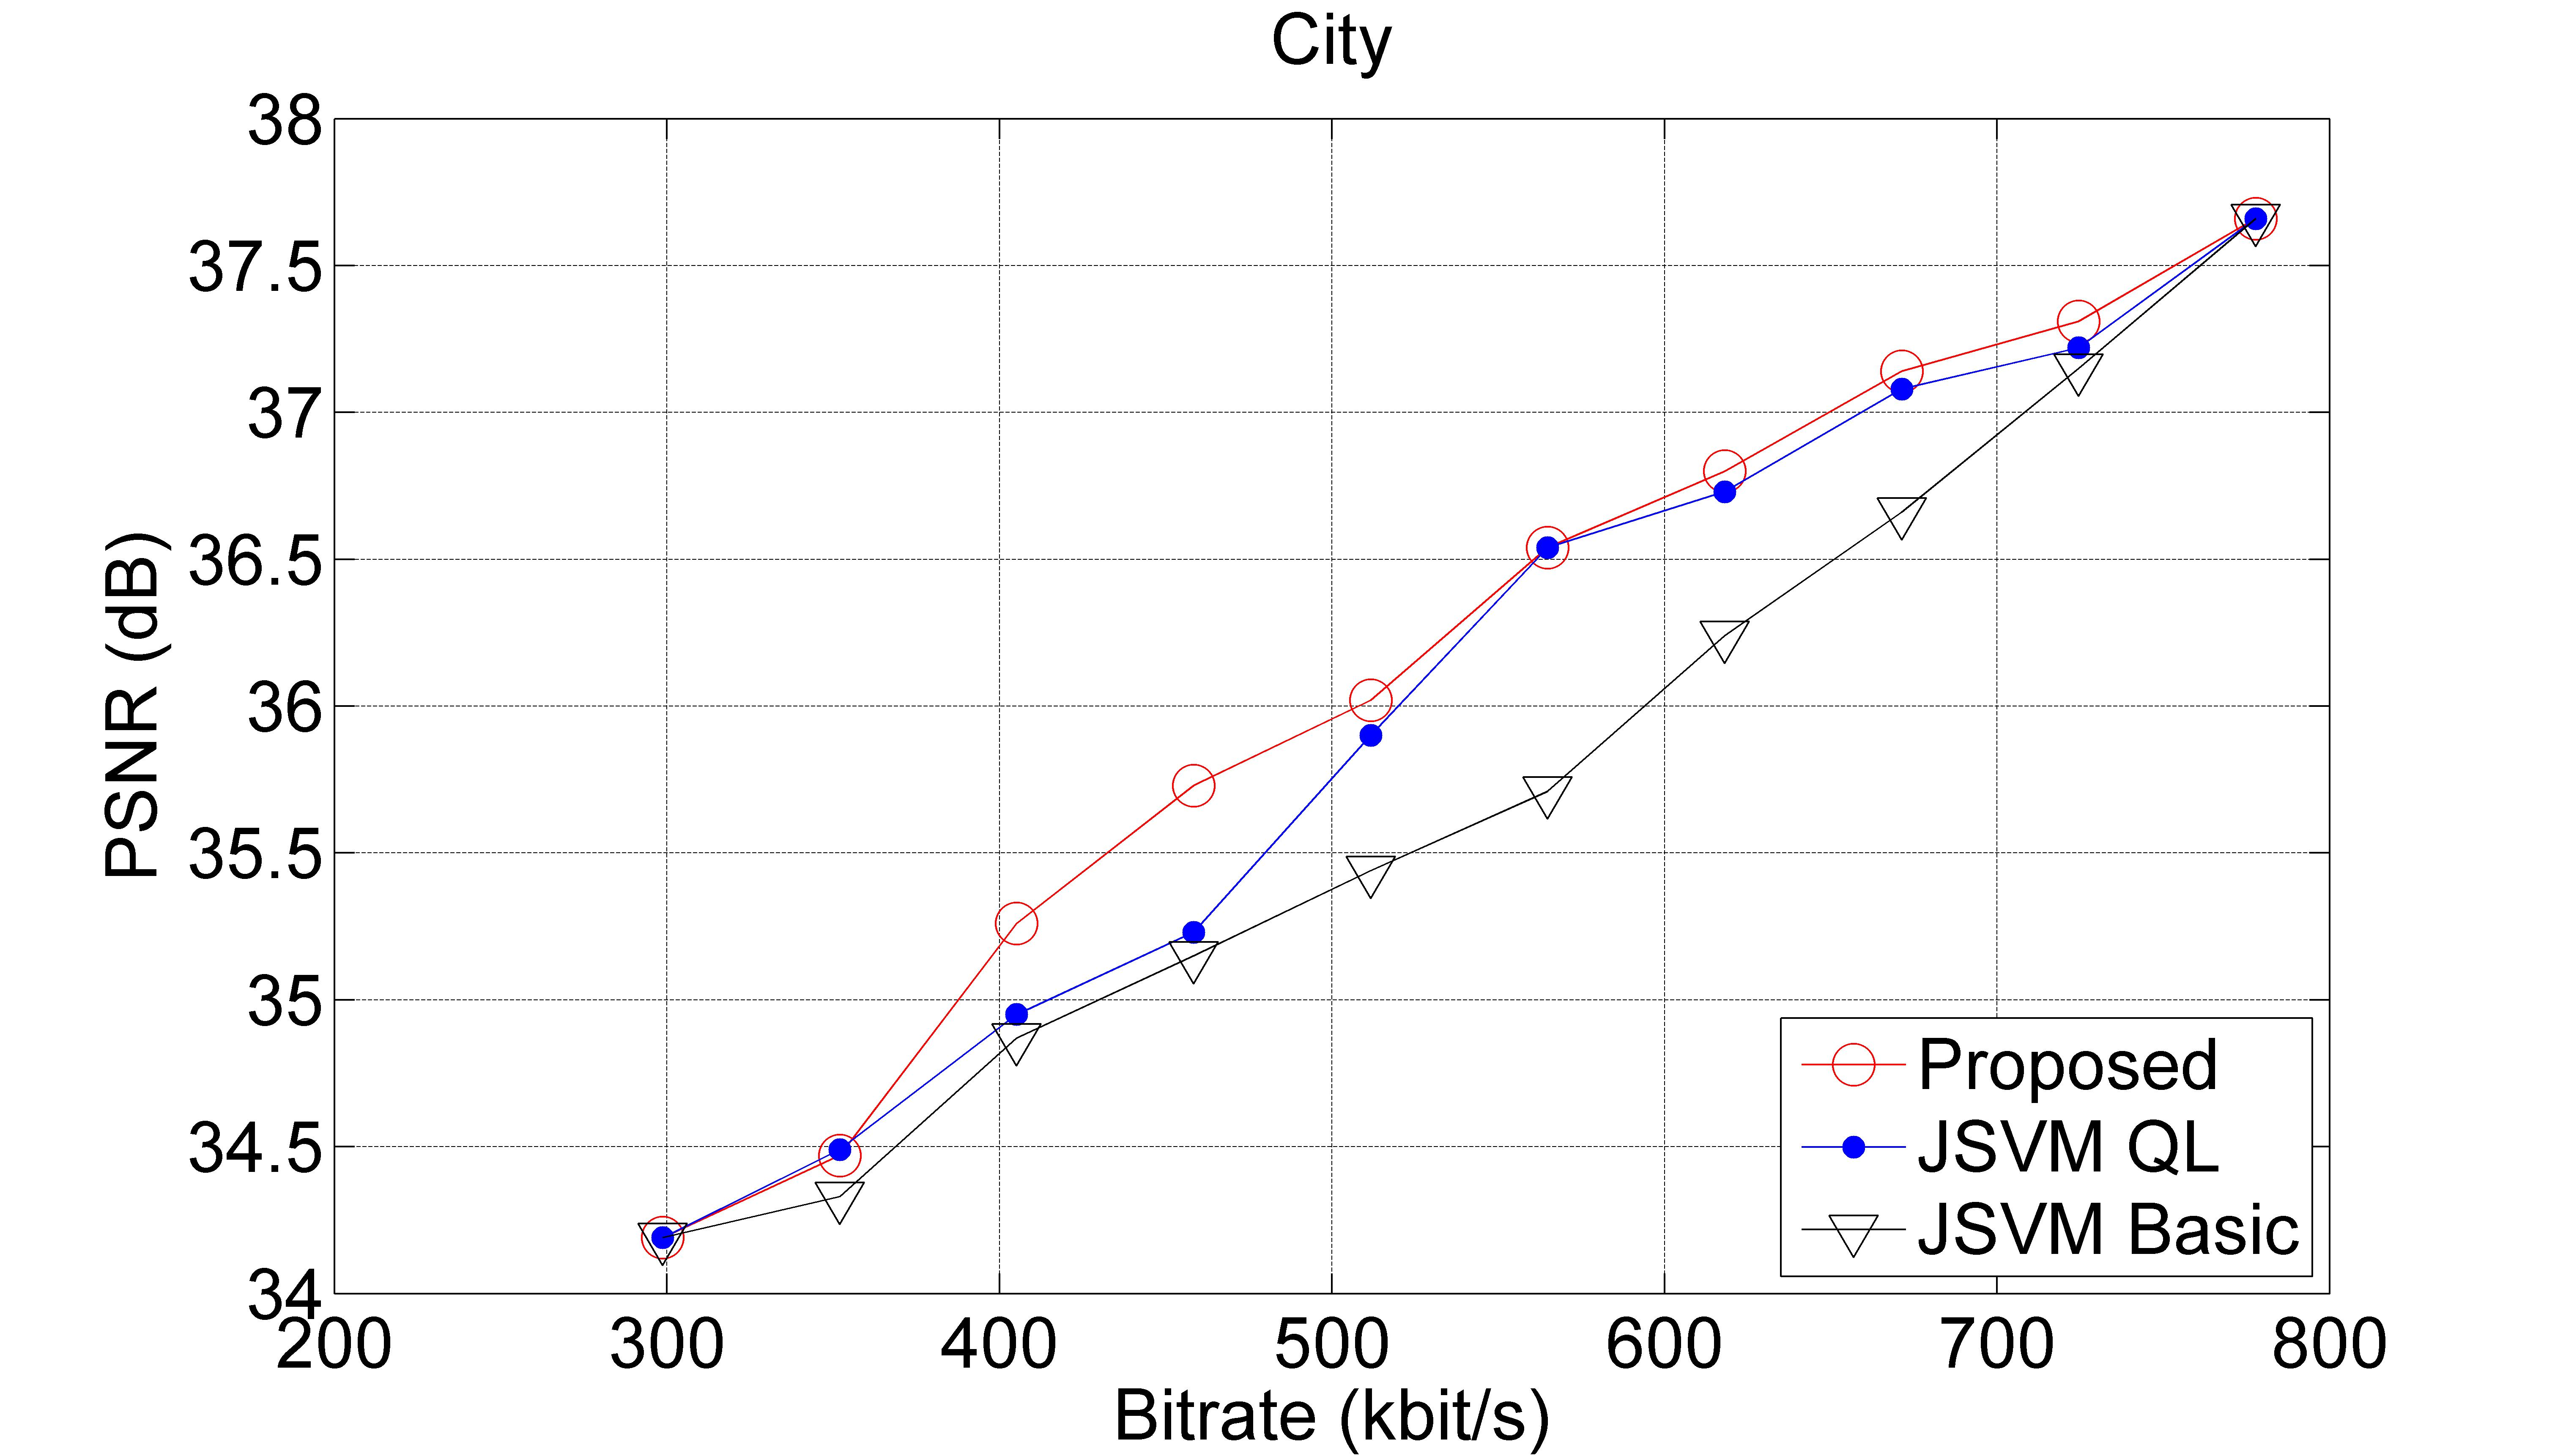
\includegraphics[width=0.5\textwidth]{figures/City.jpg}
		\label{fig:City}}
	\qquad
	\subfloat[Crew]{
		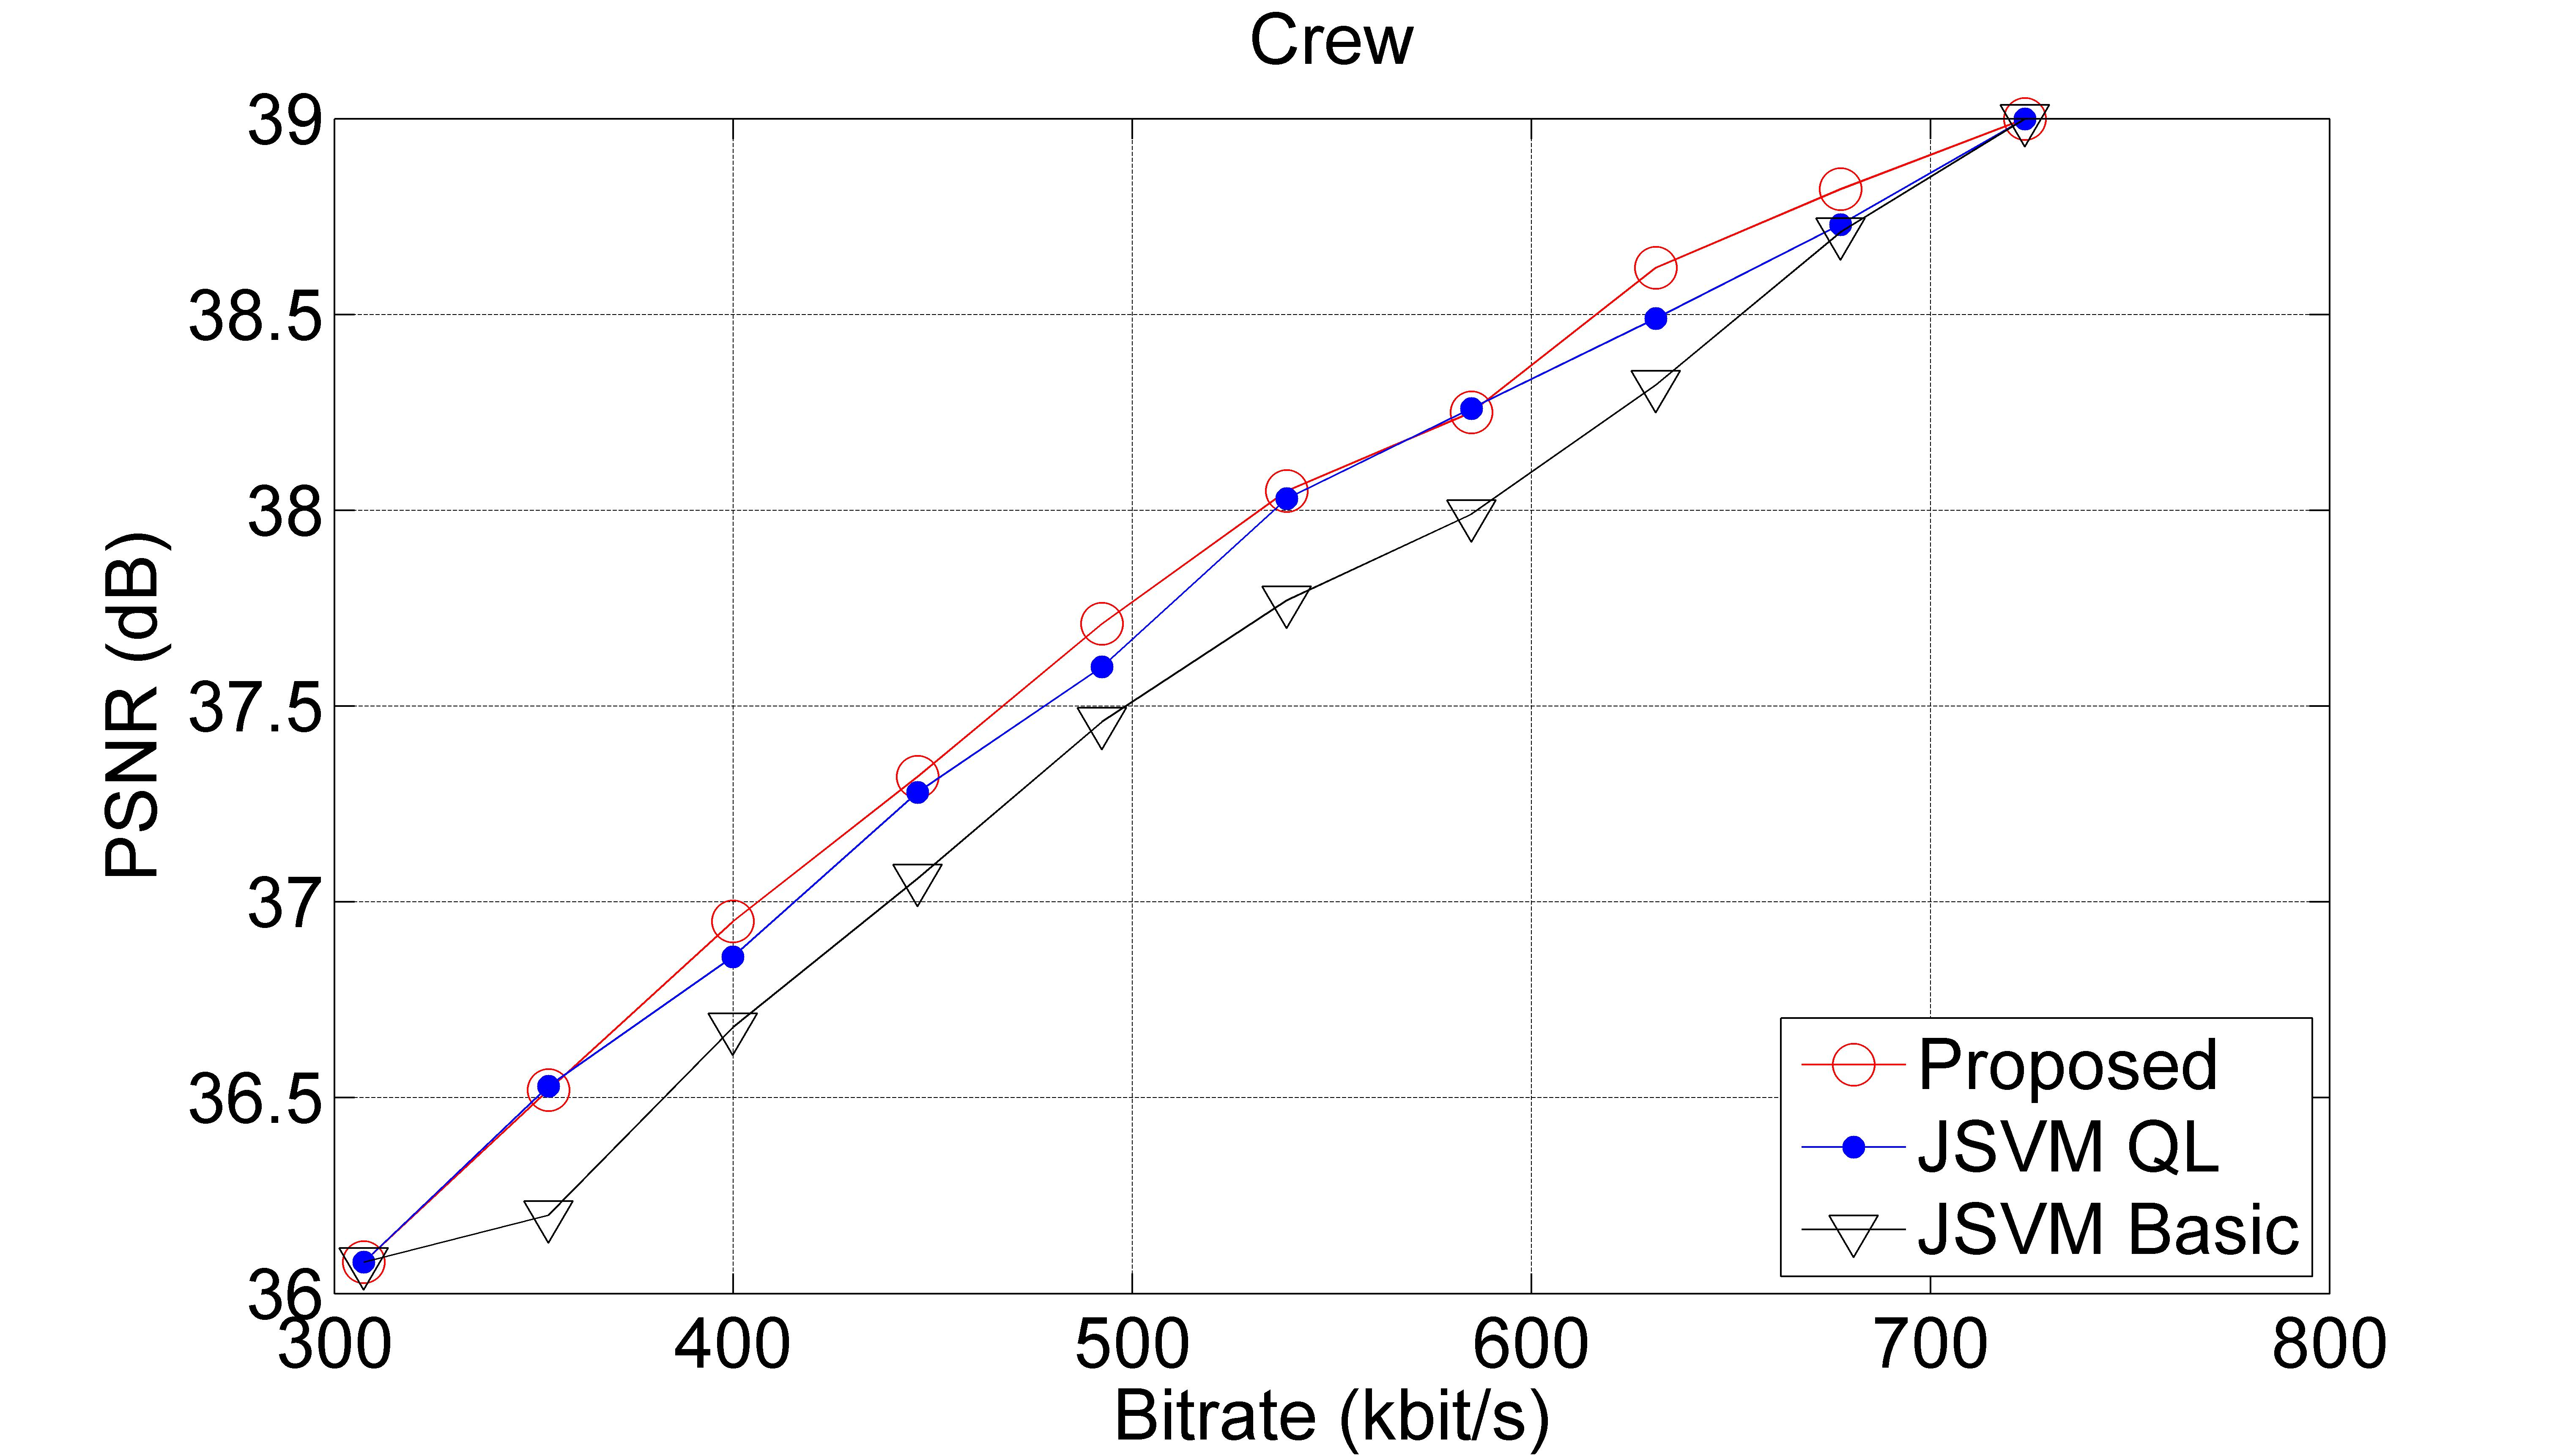
\includegraphics[width=0.5\textwidth]{figures/Crew.jpg}
		\label{fig:Crew}}
	\subfloat[Harbour]{
		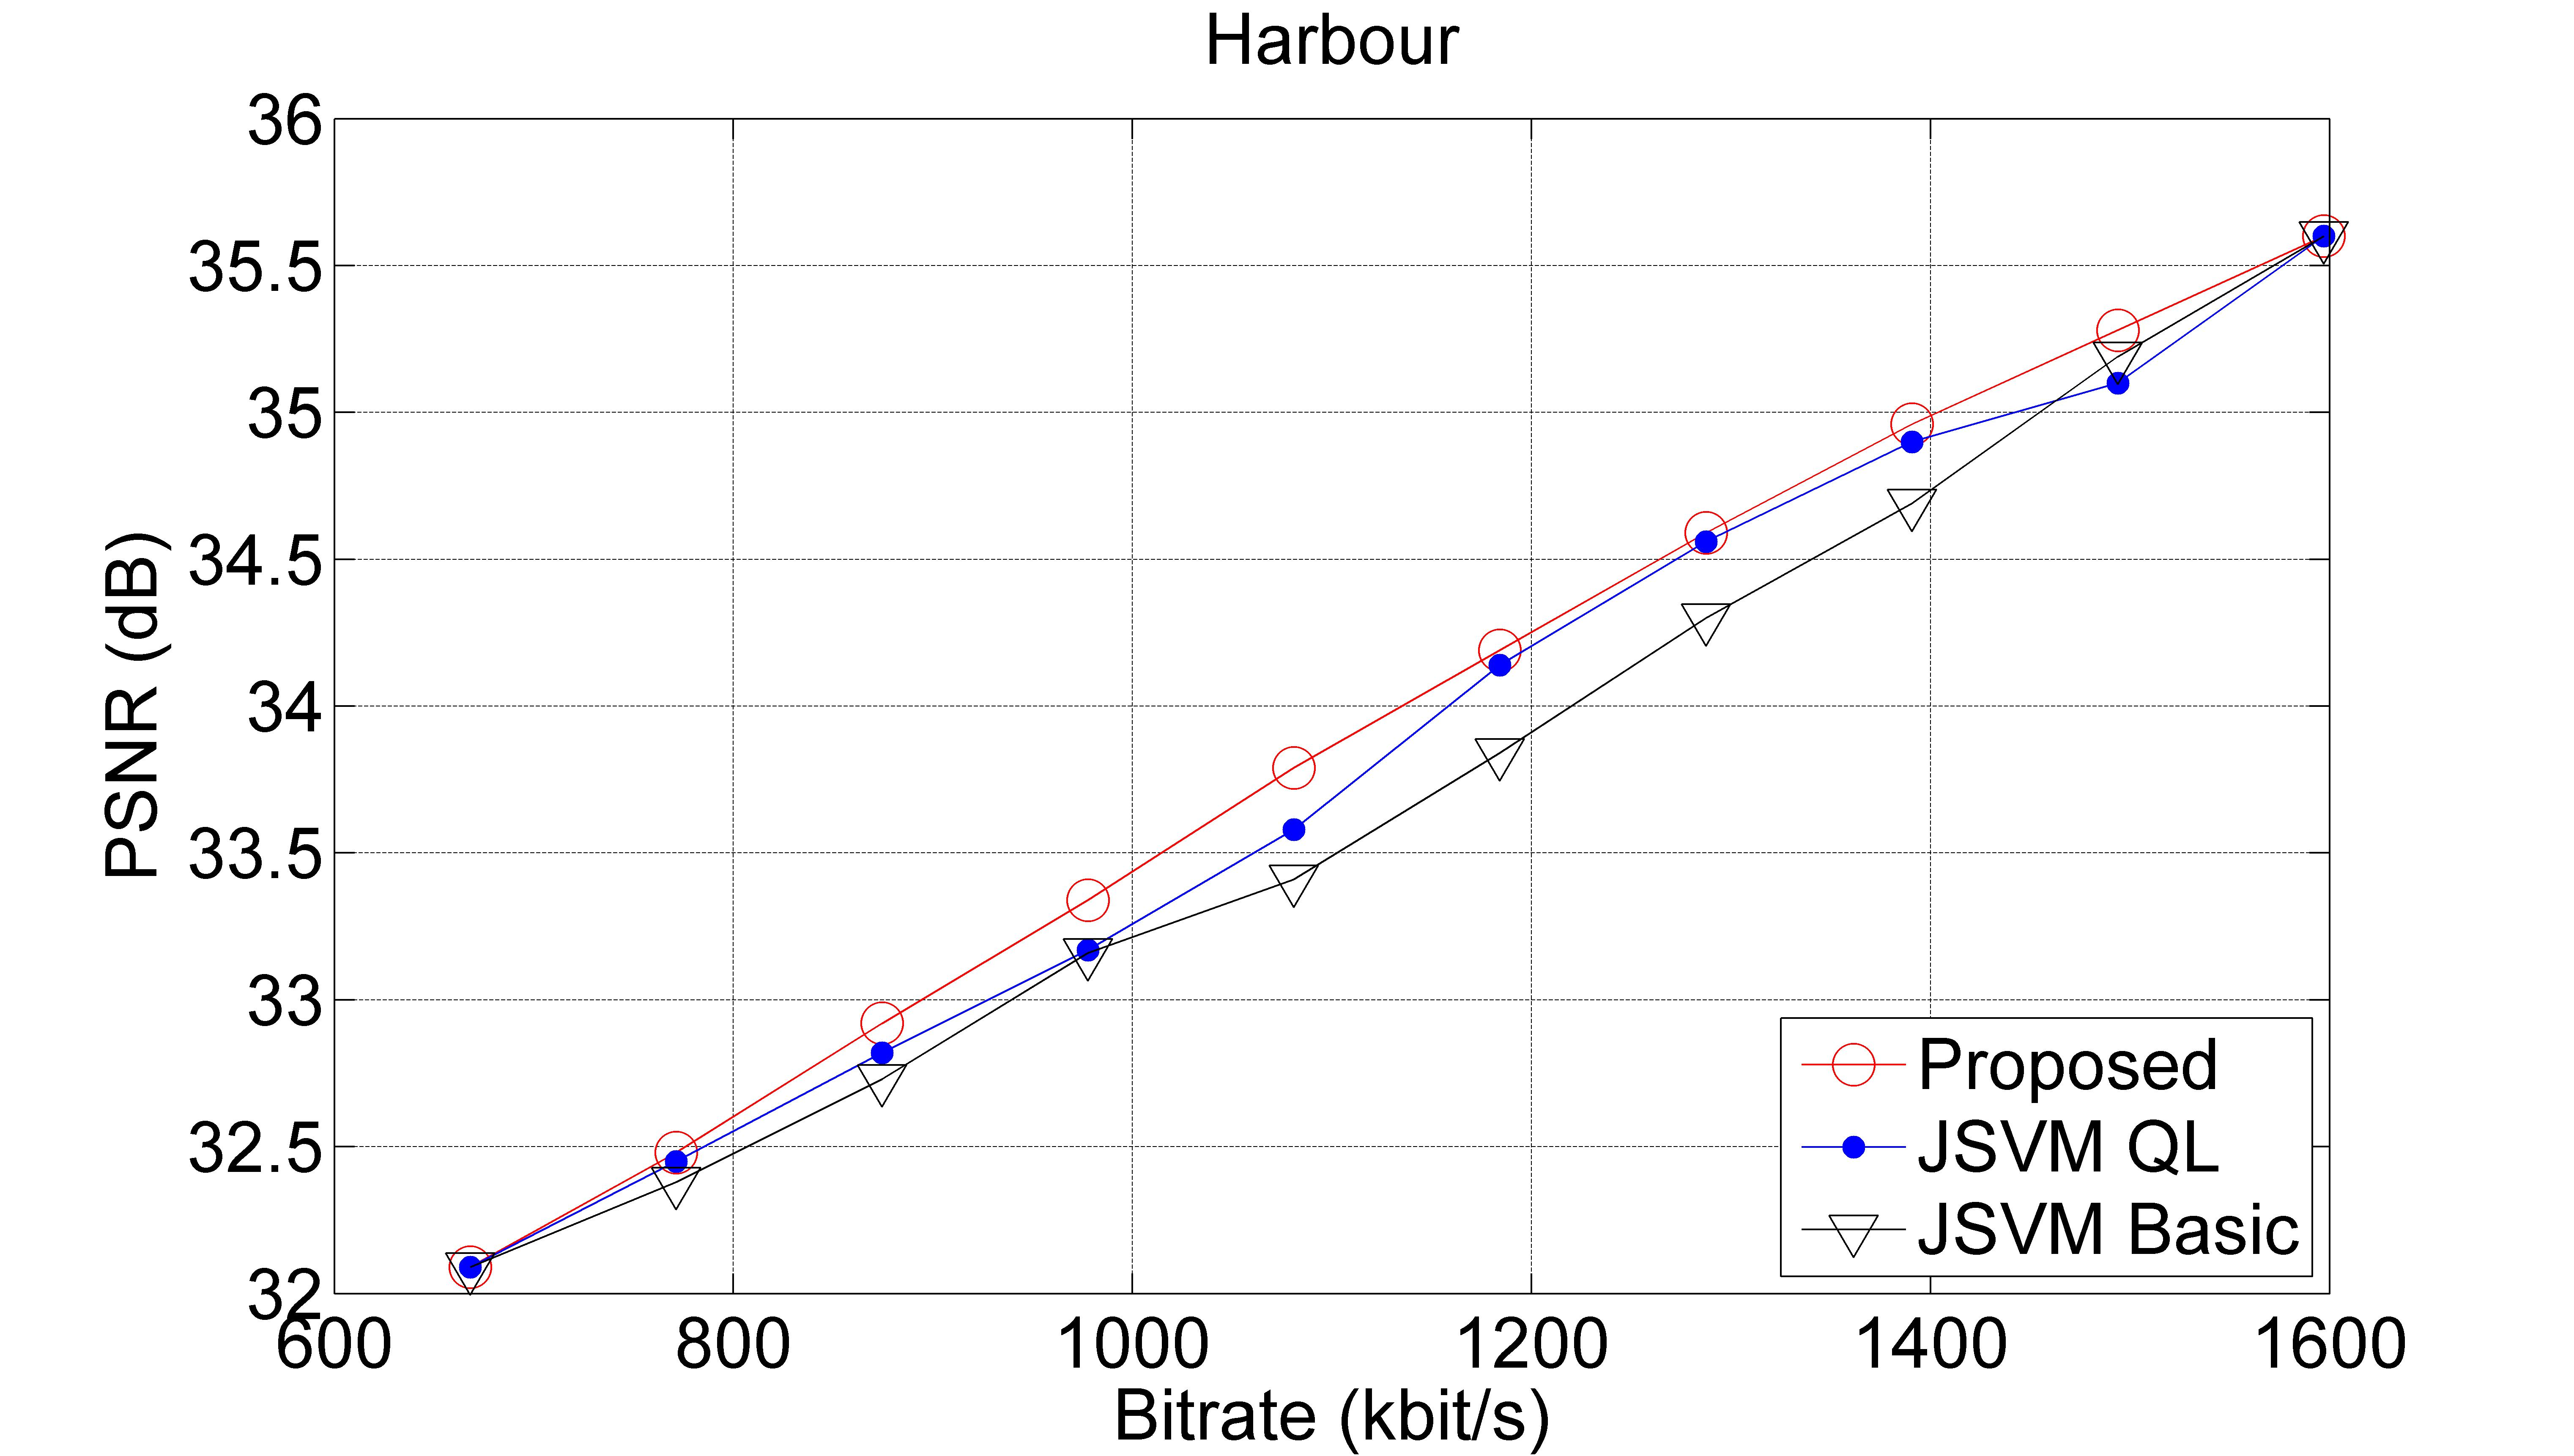
\includegraphics[width=0.5\textwidth]{figures/Harbour.jpg}
		\label{fig:Harbour}}
	\qquad
	\subfloat[Football]{
		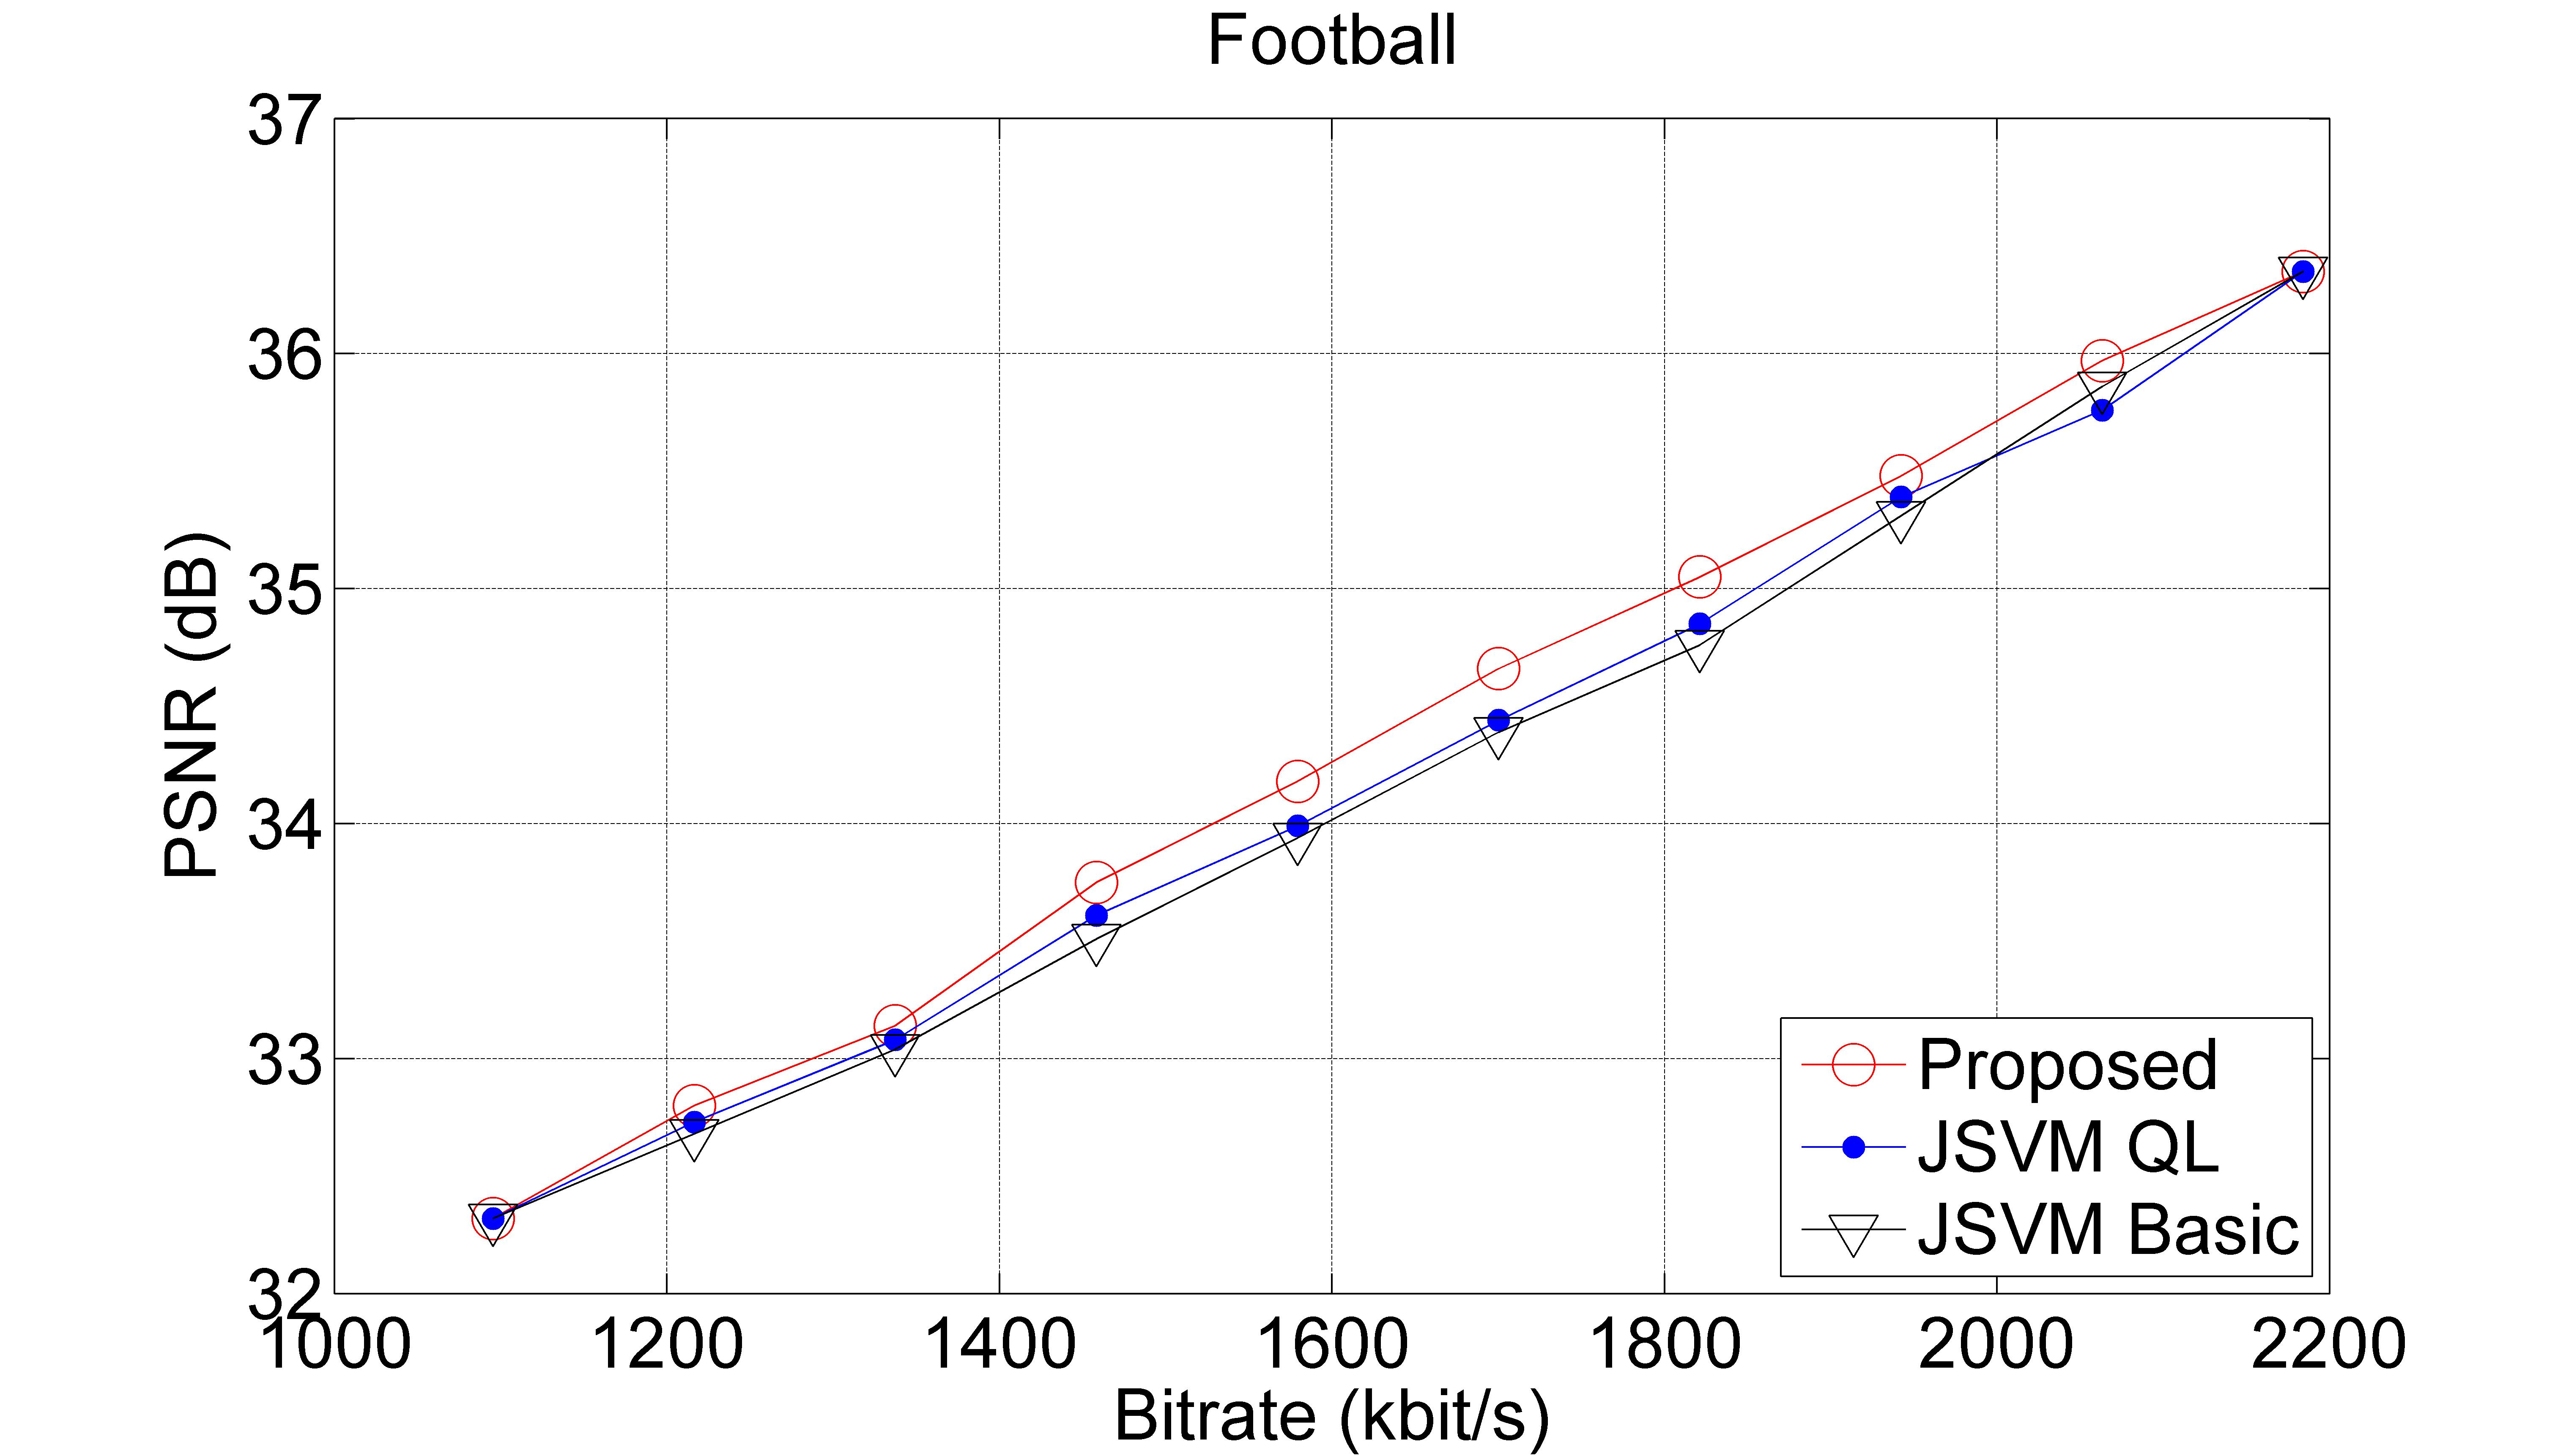
\includegraphics[width=0.5\textwidth]{figures/Football.jpg}
		\label{fig:Football}}
	\subfloat[Foreman]{
		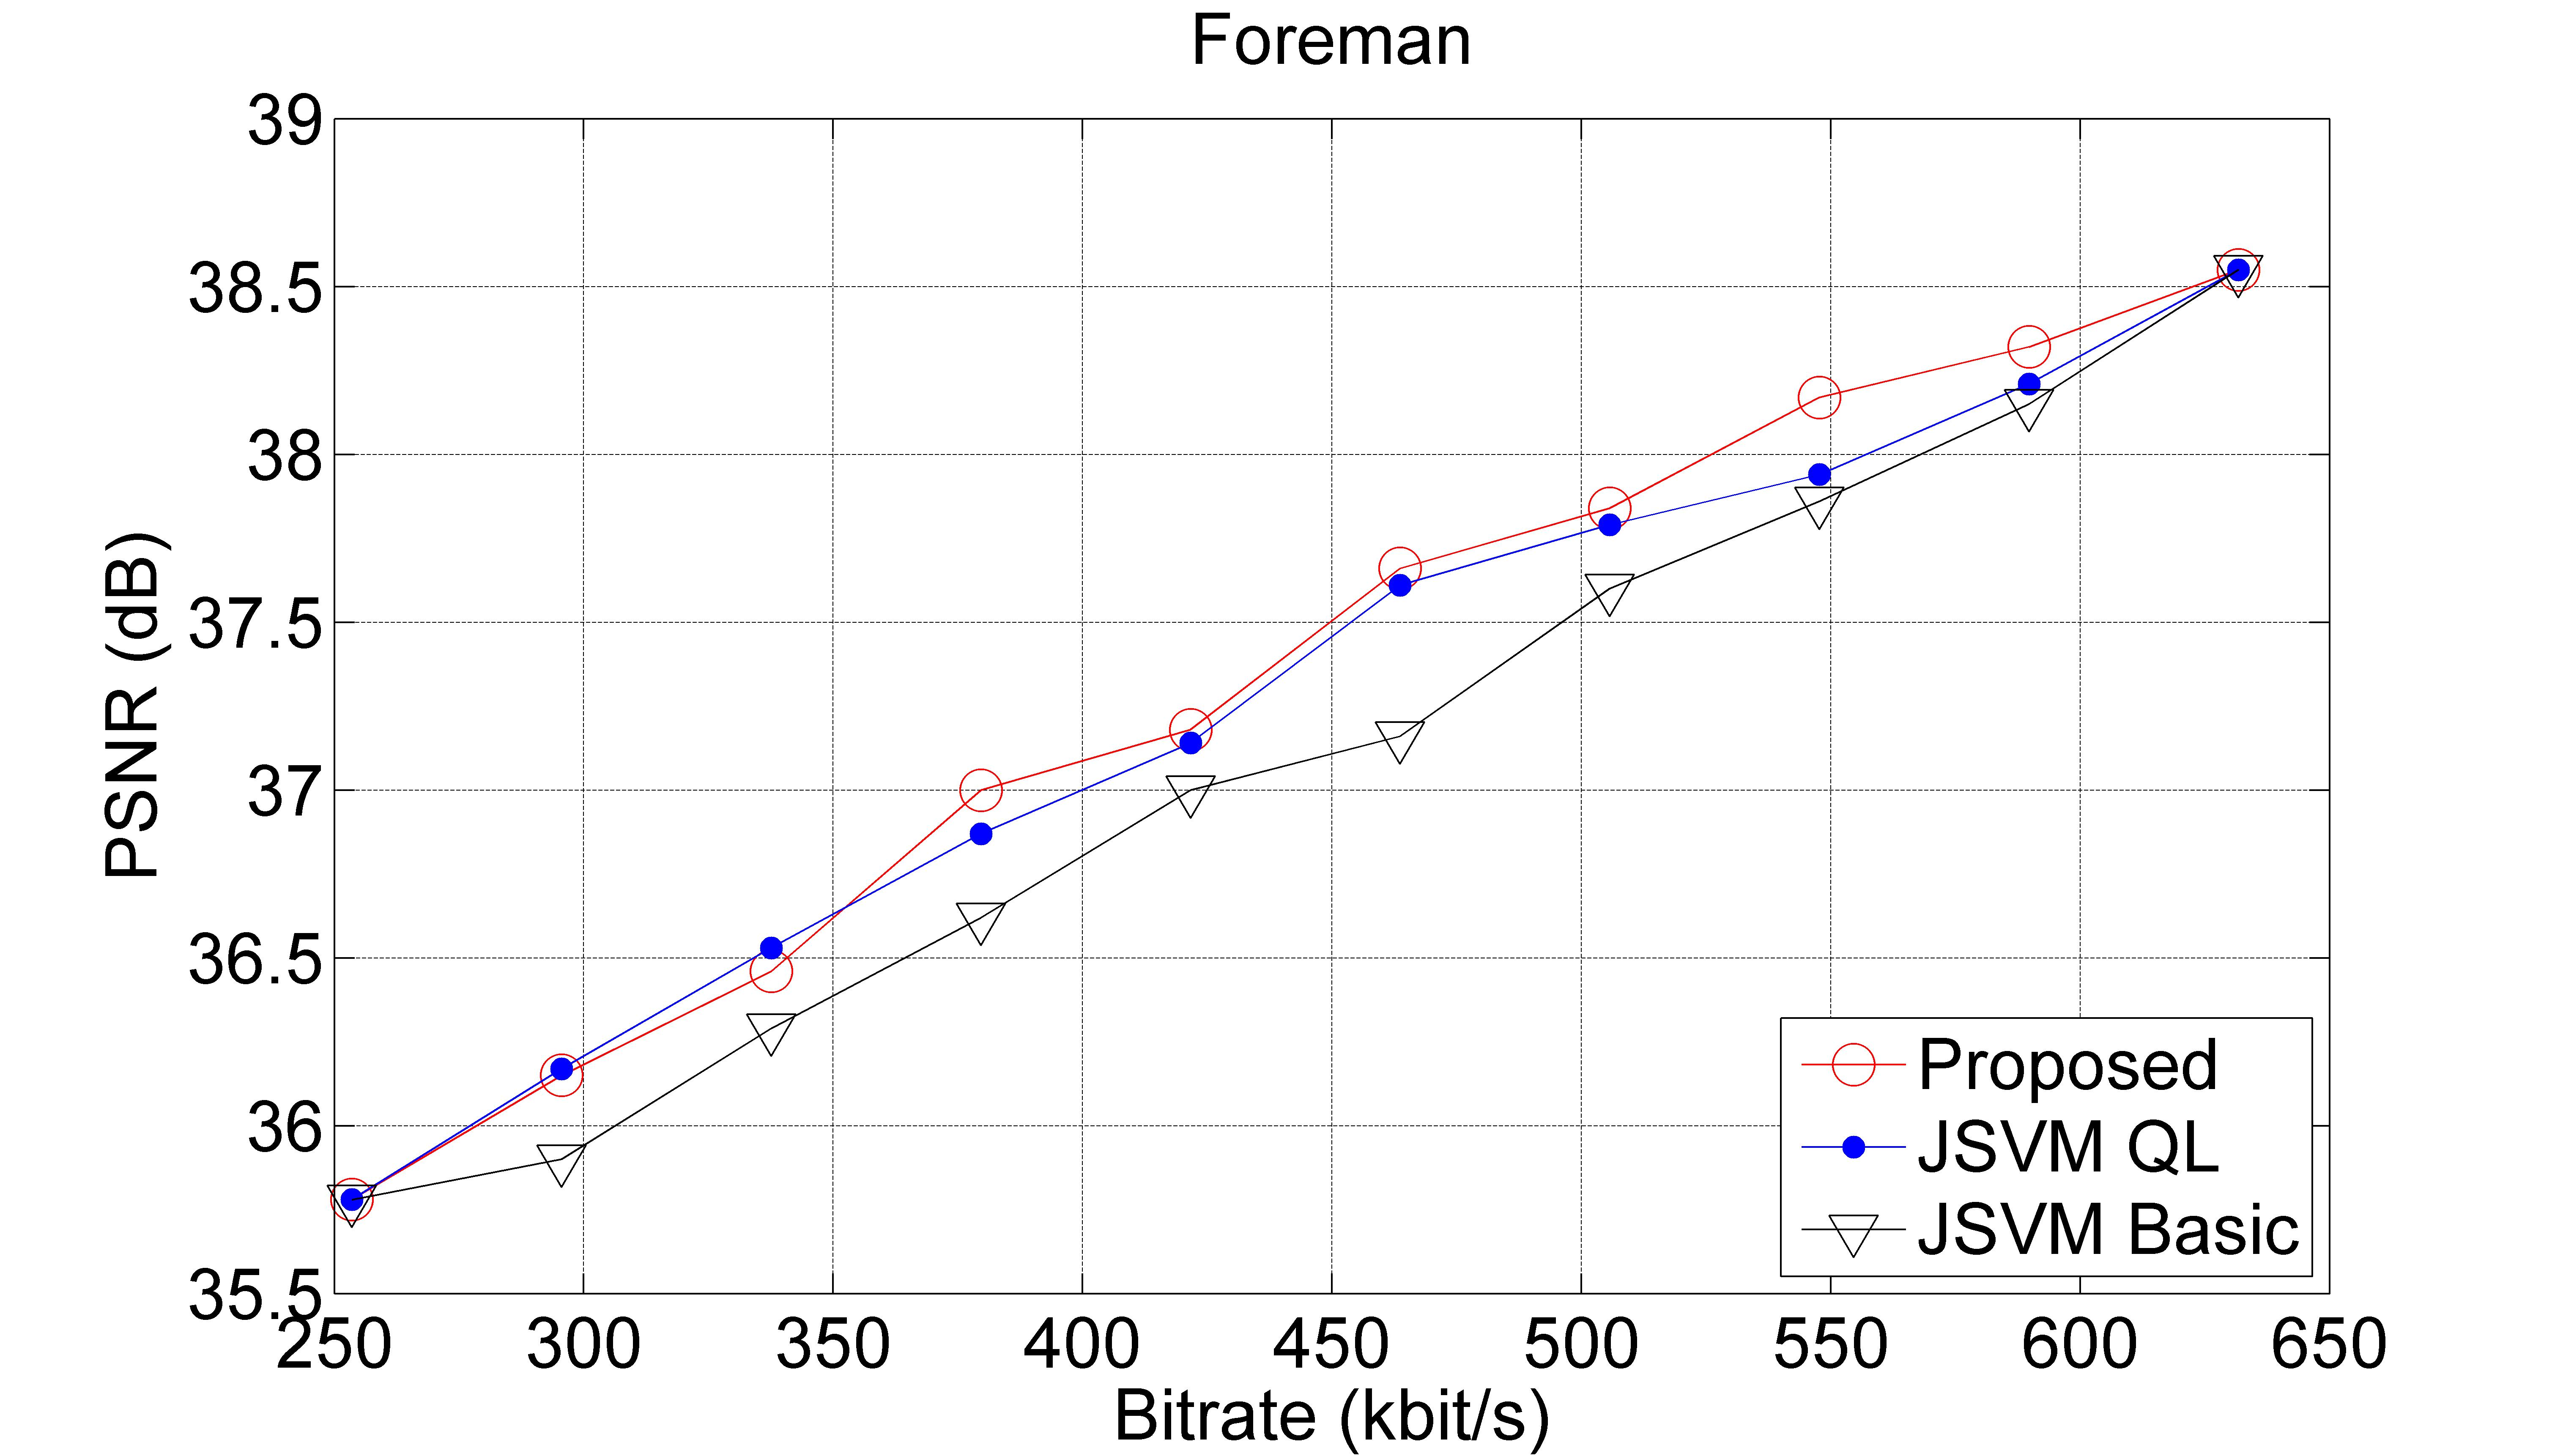
\includegraphics[width=0.5\textwidth]{figures/Foreman.jpg}
		\label{fig:Foreman}}
	\qquad
	\subfloat[Mobile]{
		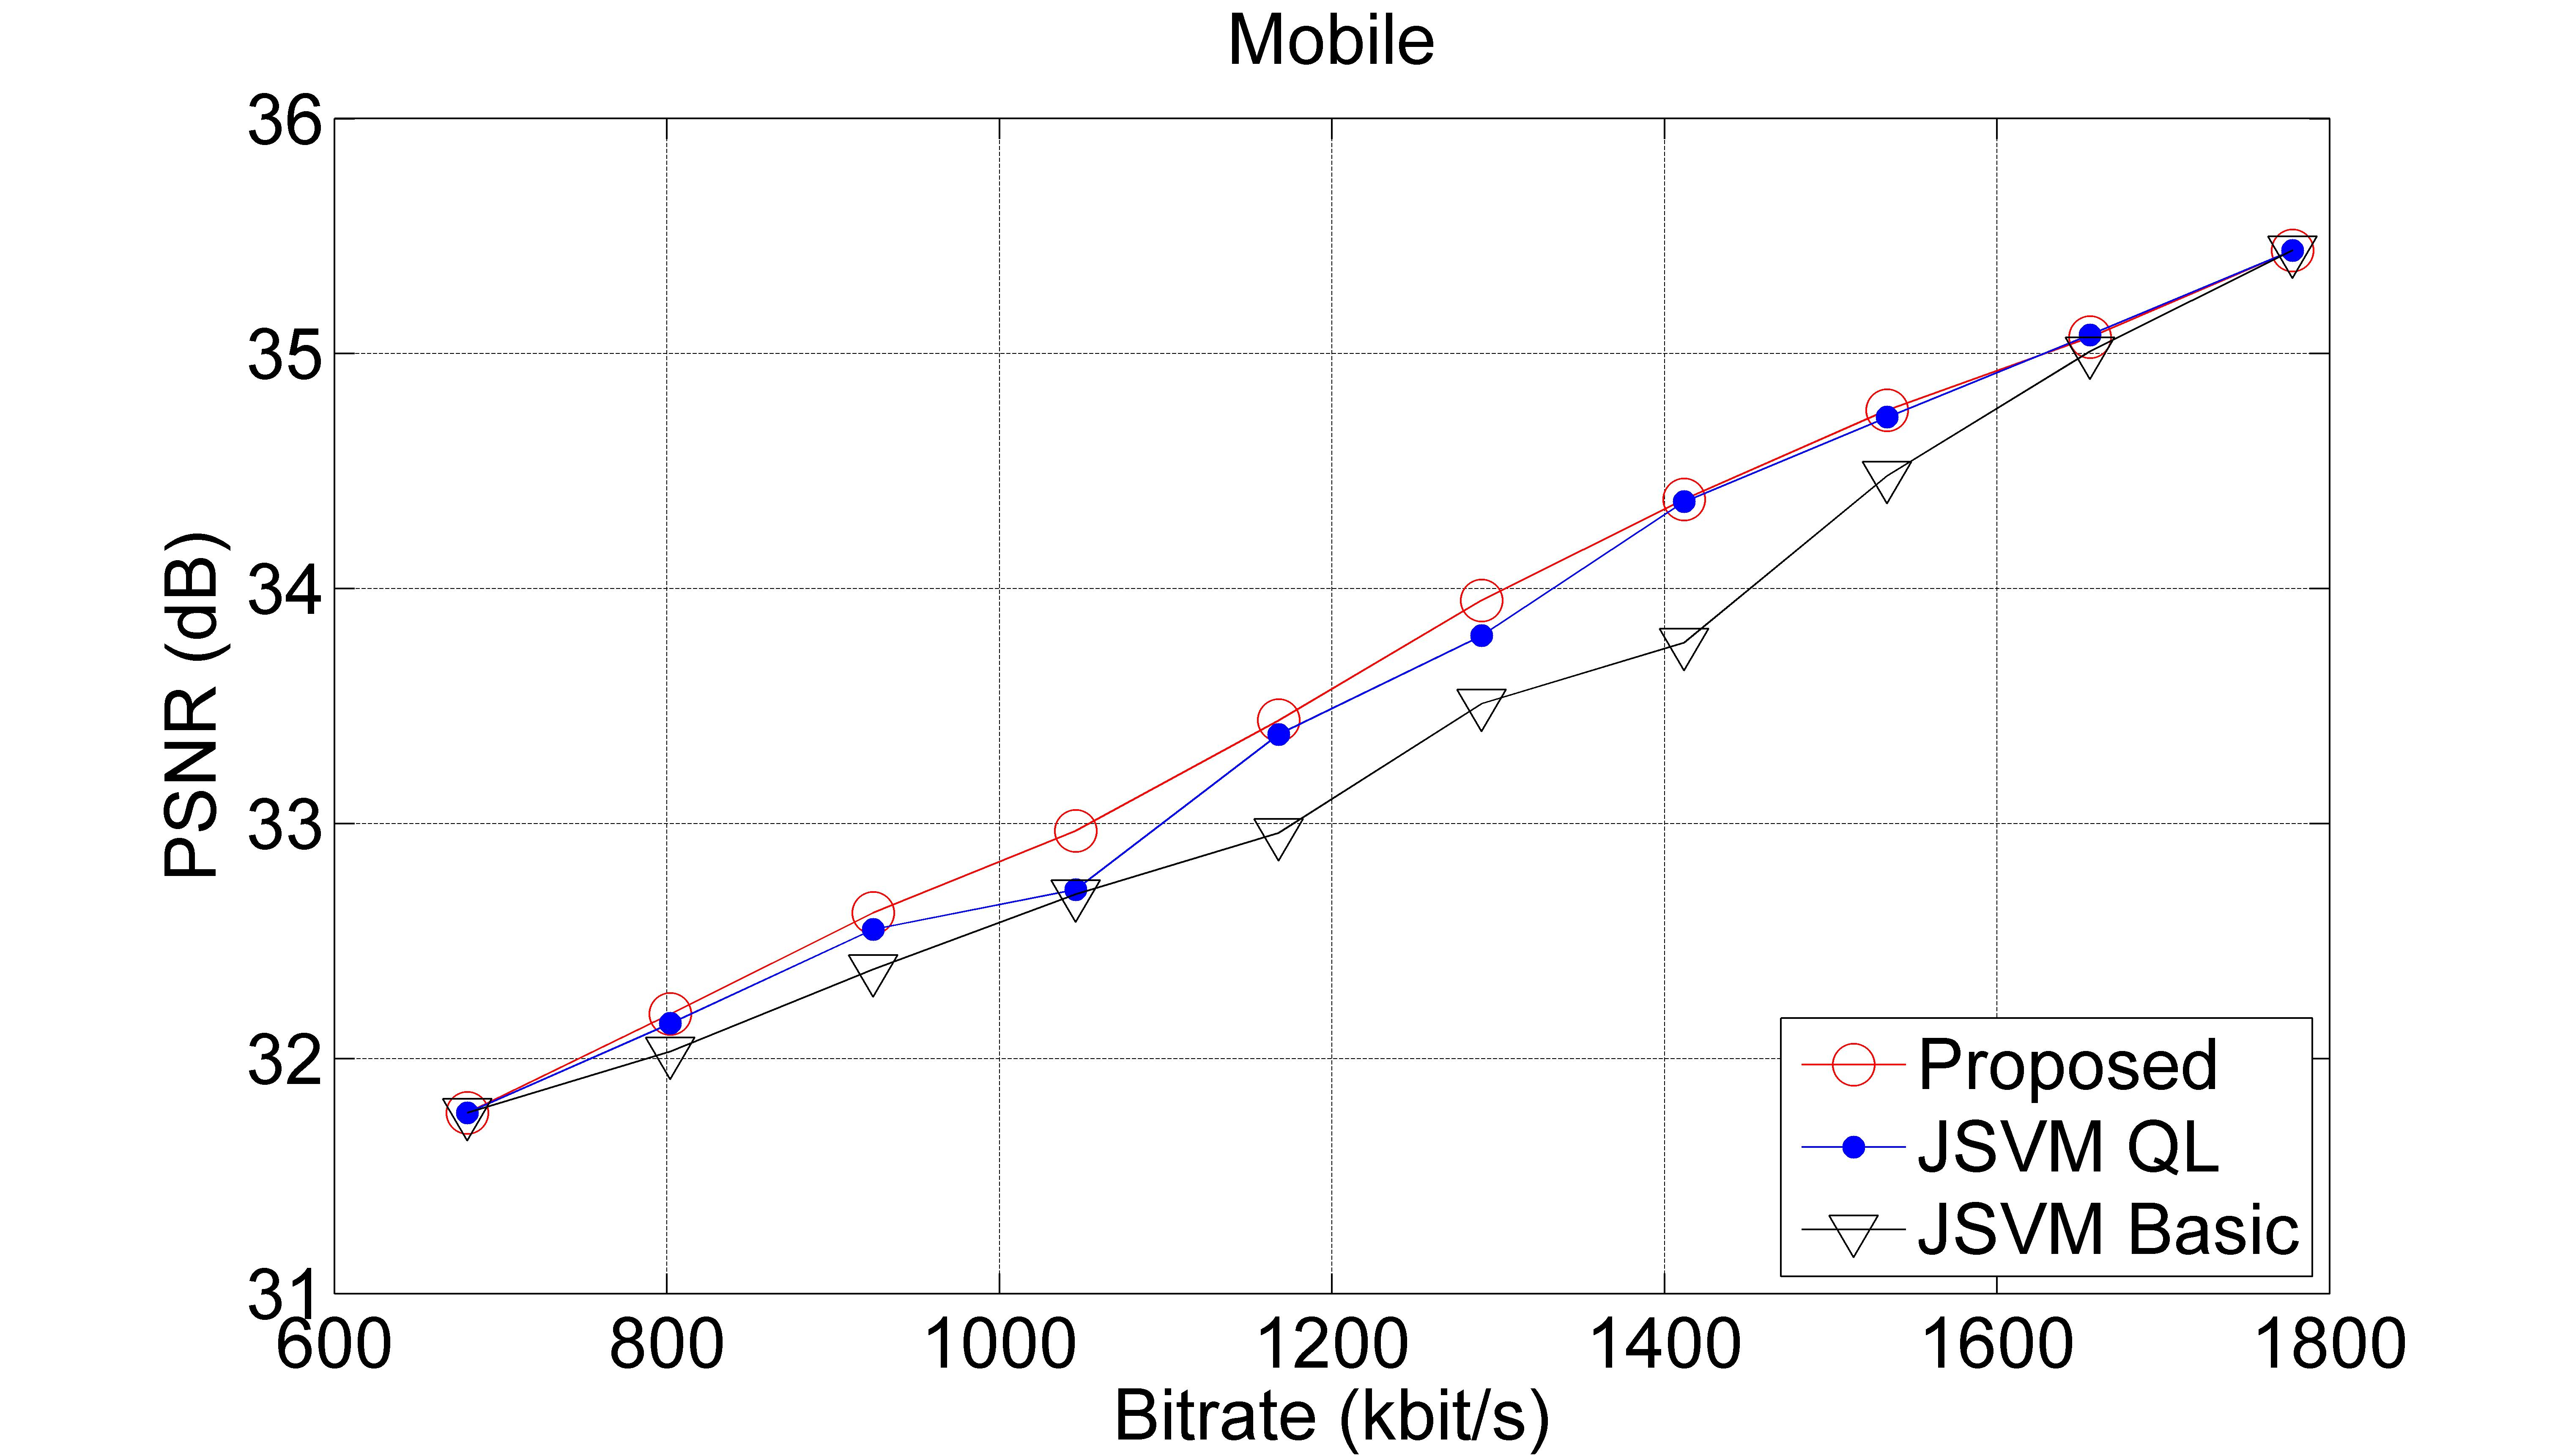
\includegraphics[width=0.5\textwidth]{figures/Mobile.jpg}
		\label{fig:Mobile}}
	\subfloat[Soccer]{
		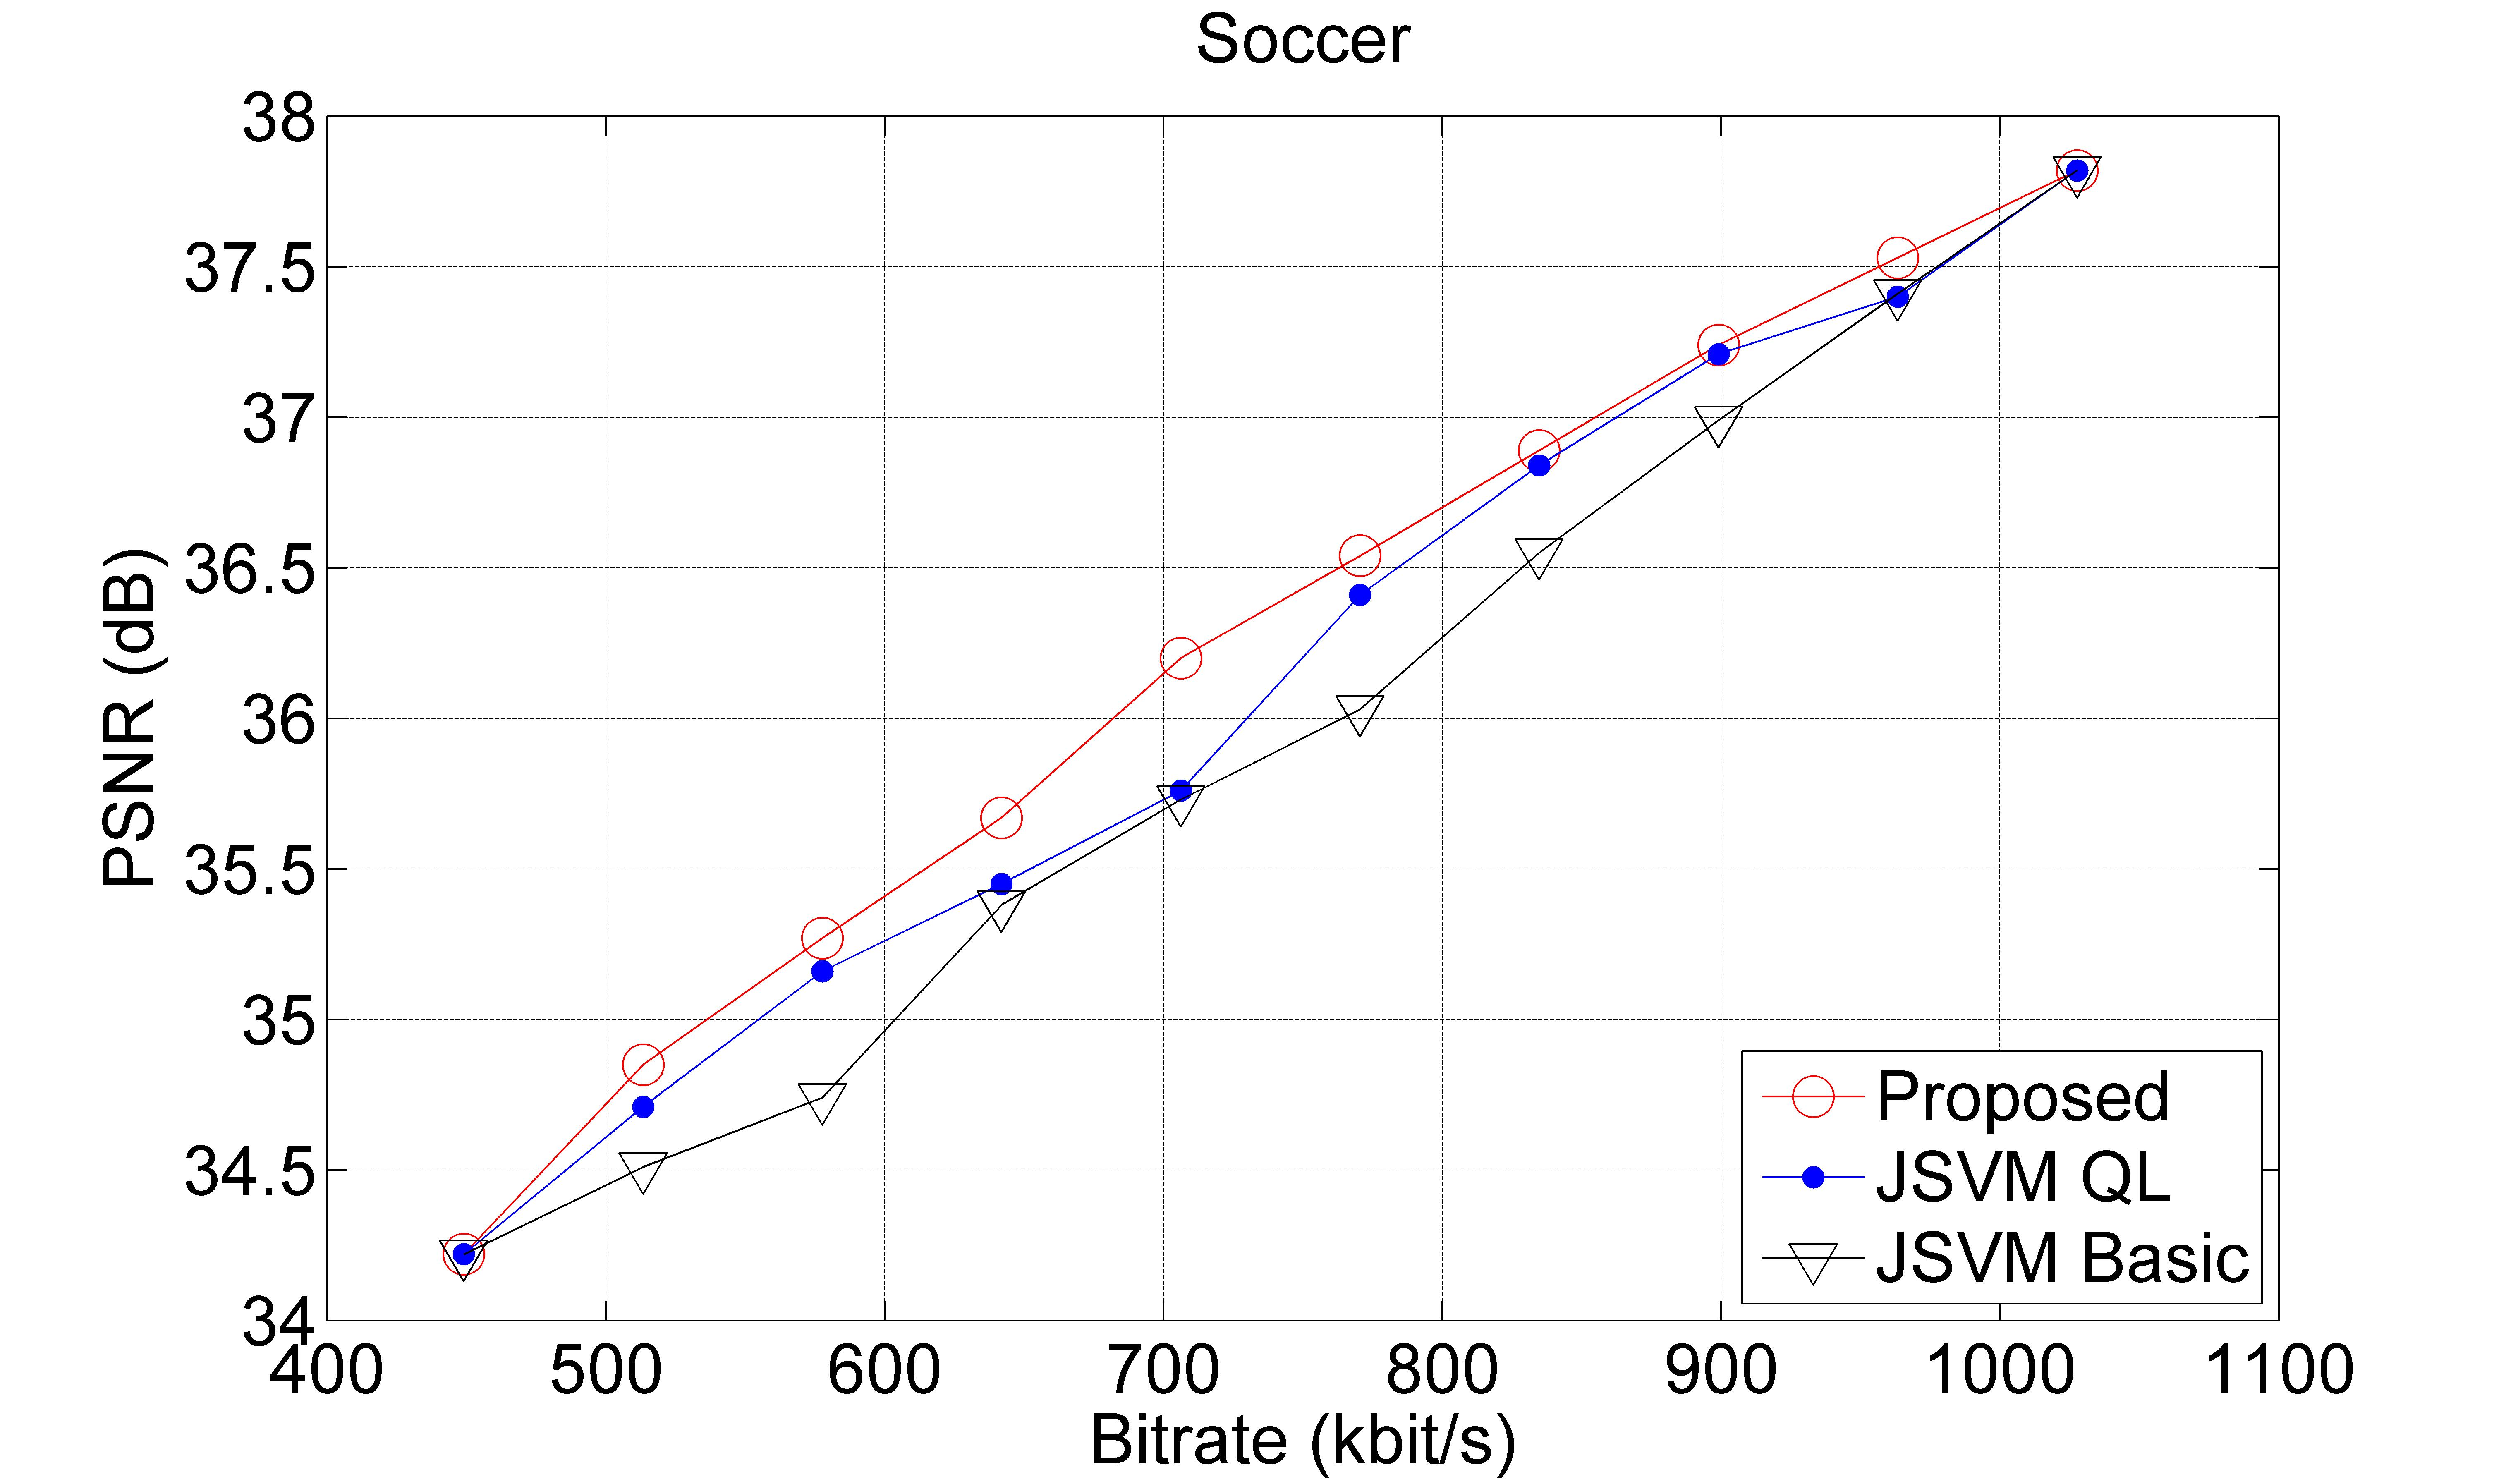
\includegraphics[width=0.5\textwidth]{figures/Soccer.jpg}
		\label{fig:Soccer}}
	\caption{三种码流截取方案的性能比较}
	\label{fig:extraction-performance}
\end{figure*}

图\ref{fig:extraction-performance}展示了全部八个测试序列的性能比较结果。可以看出,本文提出的方法对应的码率失真曲线几乎总是在最上方。这意味着在同样的码率限制下,本文提出的算法能取得更好的视频质量。注意到率失真曲线的第一个和最后一个点分别对应着最大程度截取和不进行截取的情况;在这两种情况下各种截取算法的结果是一样的,因此图中的三条曲线在这些点重合。

表\ref{tab:extraction-gain}列出了本文提出的截取方案相对于比较对象的PSNR提升。对于每一个测试序列,10个码率点的最大和平均PSNR提升都列了出来。可以看到,我们的方法相对于JSVM有明显的性能优势。该表中还列出了当优化窗口设置为48帧(也就是6个GOP)时的结果,证明了通过增大优化窗口确实能提升性能。不过在实际系统中,窗口大小还需考虑其他因素,并非能任意增大(参见\ref{subsec:priority-assign}小节末尾的分析)。

\begin{table*}[t]
	\centering
	\caption{本文提出的截取方案相比于JSVM的PSNR提升}
	\label{tab:extraction-gain}
	\small
	\begin{minipage}{1.0\linewidth}
		% \renewcommand{\thefootnote}{\thempfootnote}
		\centering
		\begin{tabular}{c|c|*{3}{p{0.9cm}<{\centering}|}*{4}{p{1.1cm}<{\centering}|}p{0.9cm}<{\centering}}
			%% |l|l| to left justify each column entry
			%% |c|c| to center each column entry
			%% use of \rule[]{}{} below opens up each row
			\hline \hline
			\multicolumn{2}{c|}{序列名} &
			{\em Bus} & {\em City} & {\em Crew} & {\em Football} & {\em Foreman} & {\em Harbour} & {\em Mobile} & {\em Soccer} \\ \hline 
			\multirow{2}{*}{JSVM QL, $K$ = 32 \footnote{\label{footnote:JSVM_QL} 与JSVM QL对比;优化窗口大小为32帧}}
			& Max\footnote{\label{footnote:max} 所有码率限制下的最大提升}
			& 0.37 & 0.50 & 0.13 & 0.22 & 0.23 & 0.19 & 0.25 & 0.44 \\ \cline{2-10}
			& Ave\footnote{\label{footnote:ave} 所有码率限制下的平均提升}
			& 0.11 & 0.11 & 0.05 & 0.12 & 0.05 & 0.05 & 0.06 & 0.13 \\ \hline
			\multirow{2}{*}{JSVM Basic, $K$ = 32}
			& Max & 0.50 & 0.83 & 0.32 & 0.29 & 0.50 & 0.34 & 0.61 & 0.53 \\ \cline{2-10}
			& Ave & 0.18 & 0.37 & 0.20 & 0.15 & 0.22 & 0.15 & 0.25 & 0.29 \\ \Xhline{2\arrayrulewidth}
			\multirow{2}{*}{JSVM QL, $K$ = 48}
			& Max & 0.36 & 0.39 & 0.27 & 0.30 & 0.30 & 0.38 & 0.21 & 0.40 \\ \cline{2-10}
			& Ave & 0.12 & 0.23 & 0.16 & 0.13 & 0.15 & 0.13 & 0.08 & 0.21 \\ \hline
			\multirow{2}{*}{JSVM Basic, $K$ = 48}
			& Max & 0.36 & 0.81 & 0.32 & 0.29 & 0.49 & 0.47 & 0.57 & 0.60 \\ \cline{2-10}
			& Ave & 0.19 & 0.40 & 0.19 & 0.17 & 0.28 & 0.22 & 0.28 & 0.42 \\ \hline
		\end{tabular}
	\end{minipage}
\end{table*}

最后需要指出,在JSVM之外的其他码流截取方法中,Maani等人的工作\supercite{Maani2009}取得了比JSVM QL高得多的性能,甚至比本文提出的方法性能还好。但是,为了得到适用于不同序列的鲁棒的模型参数,该工作中的方法需要更多的计算量去训练。而本文提出的方法所需计算量总是与JSVM相当的。据我们所知,在不显著增加计算量的情况下,码流截取很难取得较大的PSNR提升。

\subsection{无参考截取实验}

\begin{figure*}[!ht]
	\centering
	\subfloat[Bus]{
		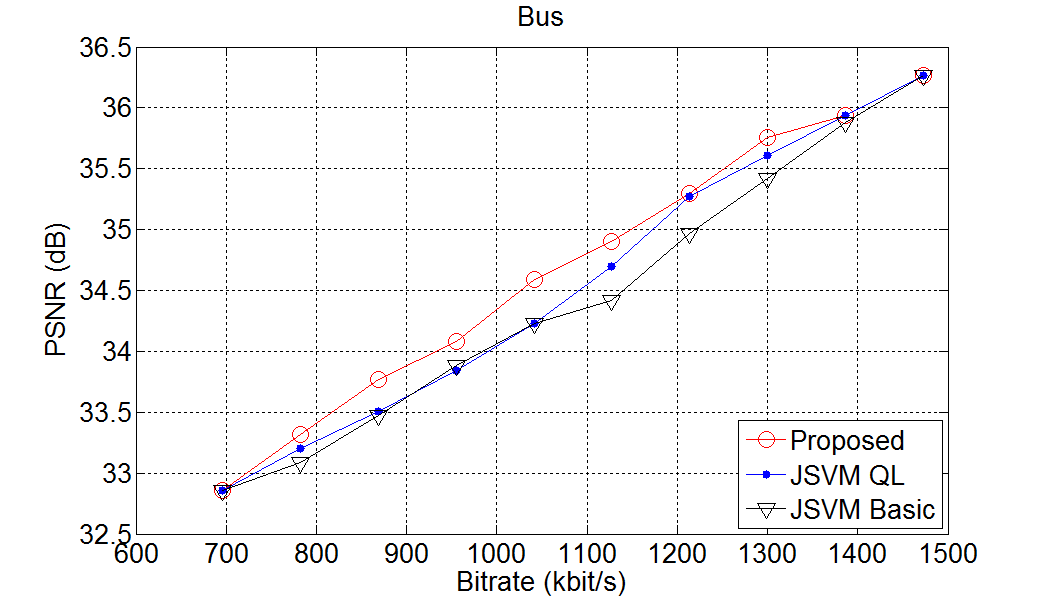
\includegraphics[width=0.5\textwidth]{figures/Bus-noref.png}}
	\subfloat[City]{
		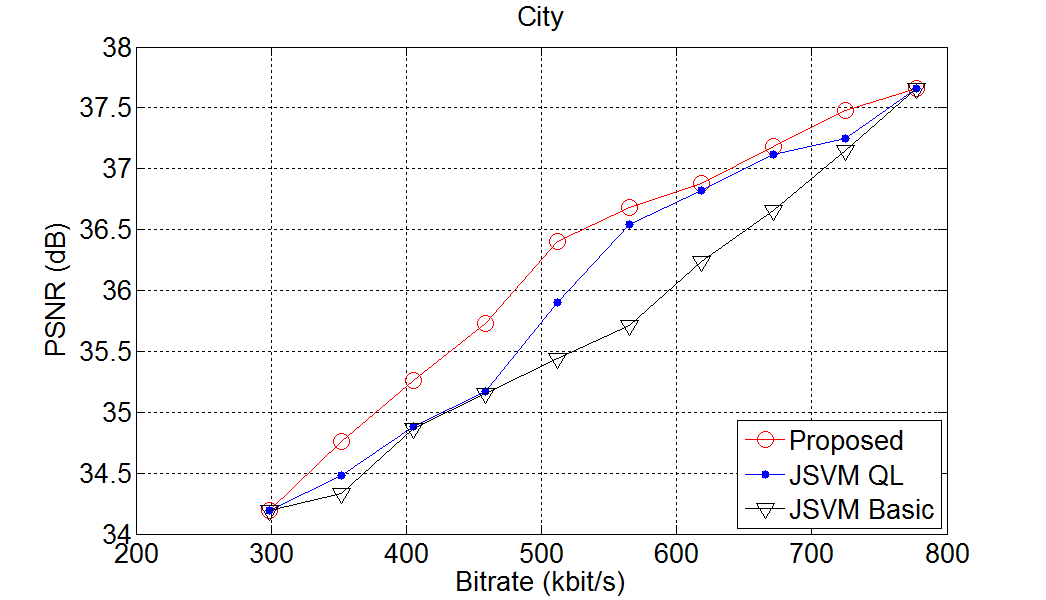
\includegraphics[width=0.5\textwidth]{figures/City-noref.png}}
	\qquad
	\subfloat[Crew]{
		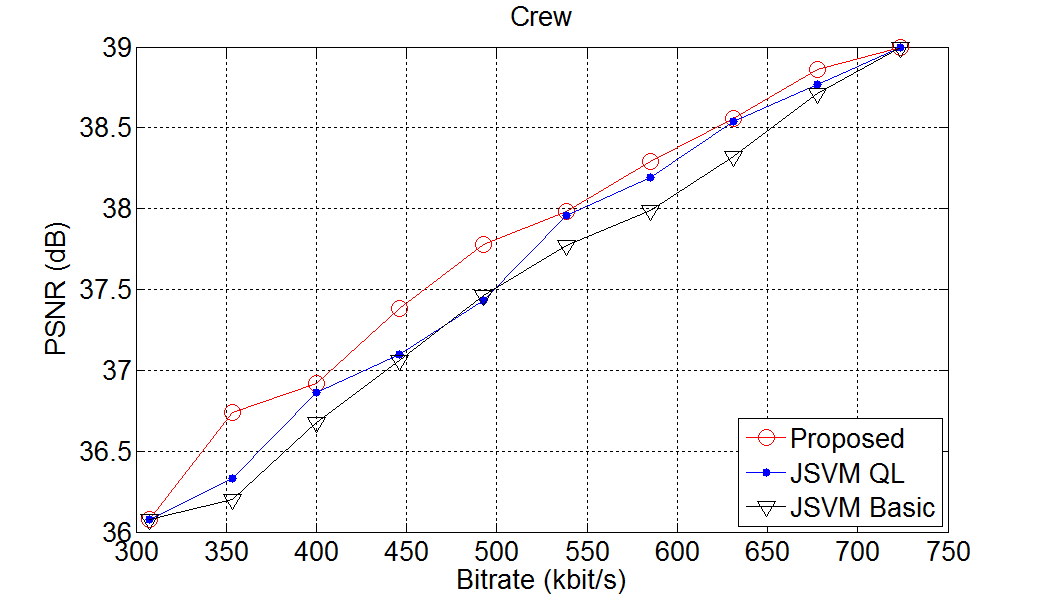
\includegraphics[width=0.5\textwidth]{figures/Crew-noref.png}}
	\subfloat[Harbour]{
		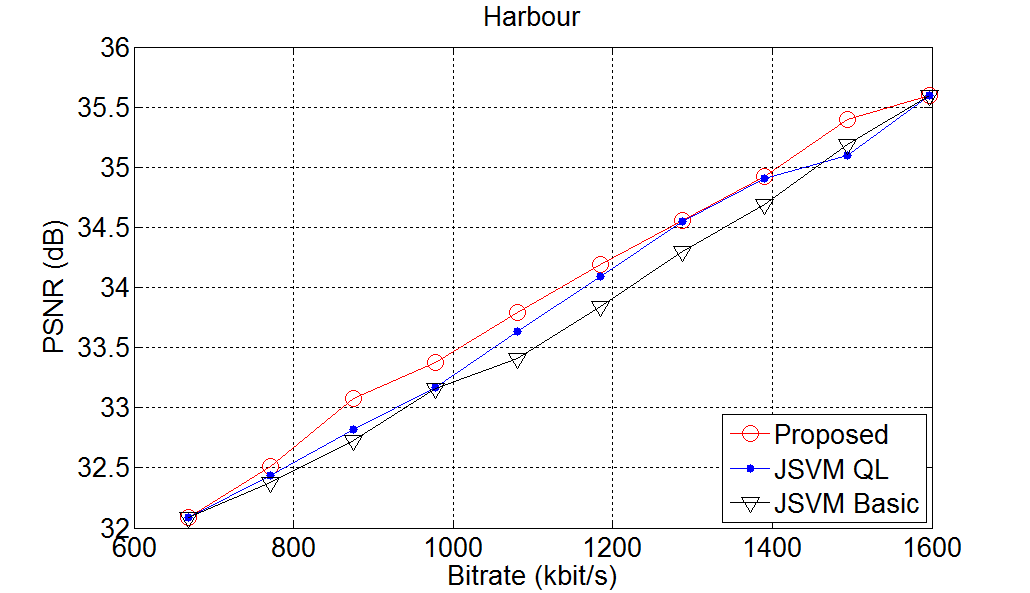
\includegraphics[width=0.5\textwidth]{figures/Harbour-noref.png}}
	\qquad
	\subfloat[Football]{
		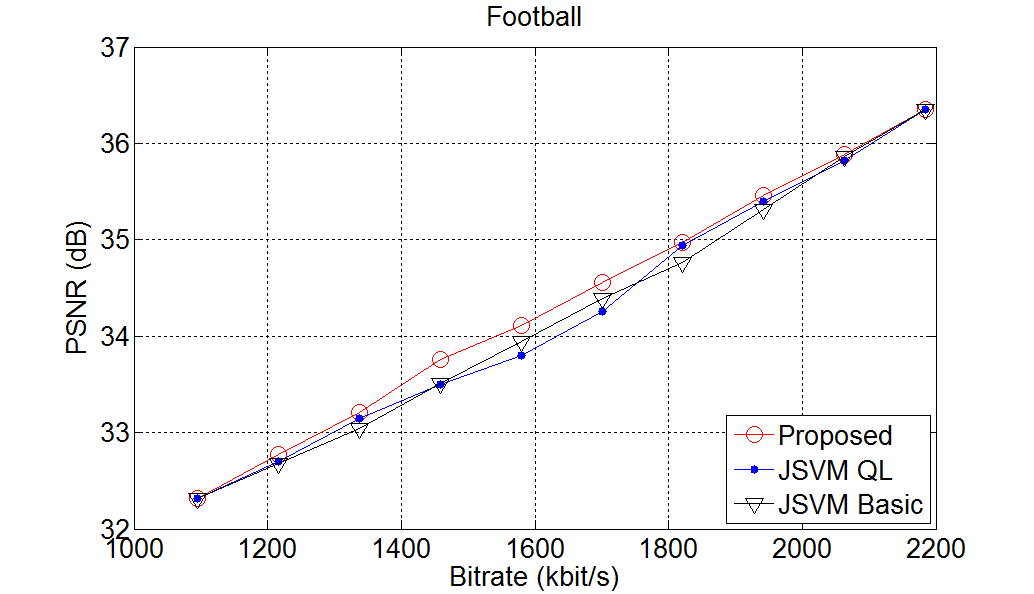
\includegraphics[width=0.5\textwidth]{figures/Football-noref.png}}
	\subfloat[Foreman]{
		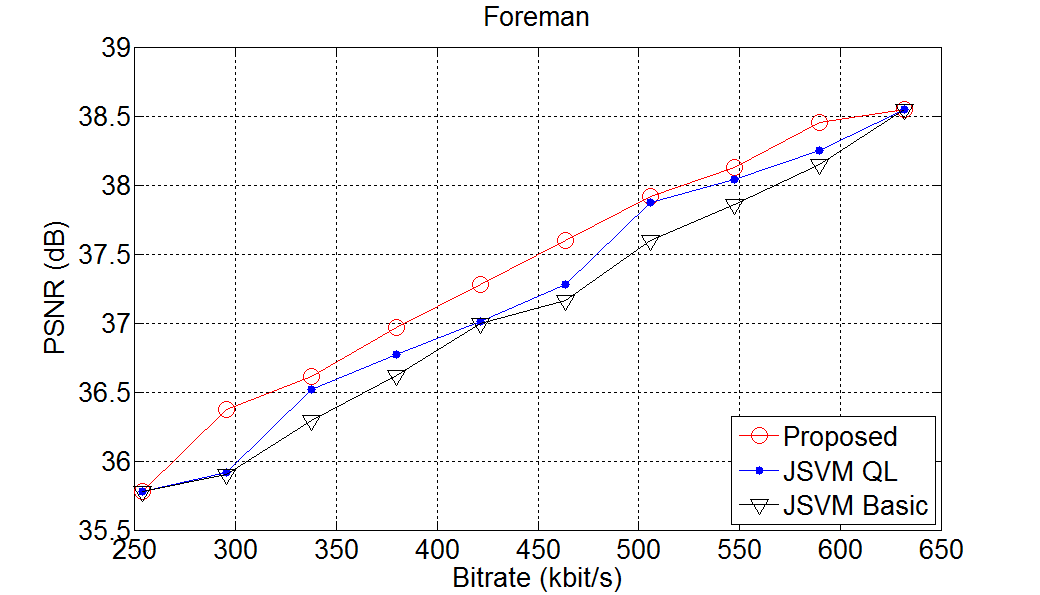
\includegraphics[width=0.5\textwidth]{figures/Foreman-noref.png}}
	\qquad
	\subfloat[Mobile]{
		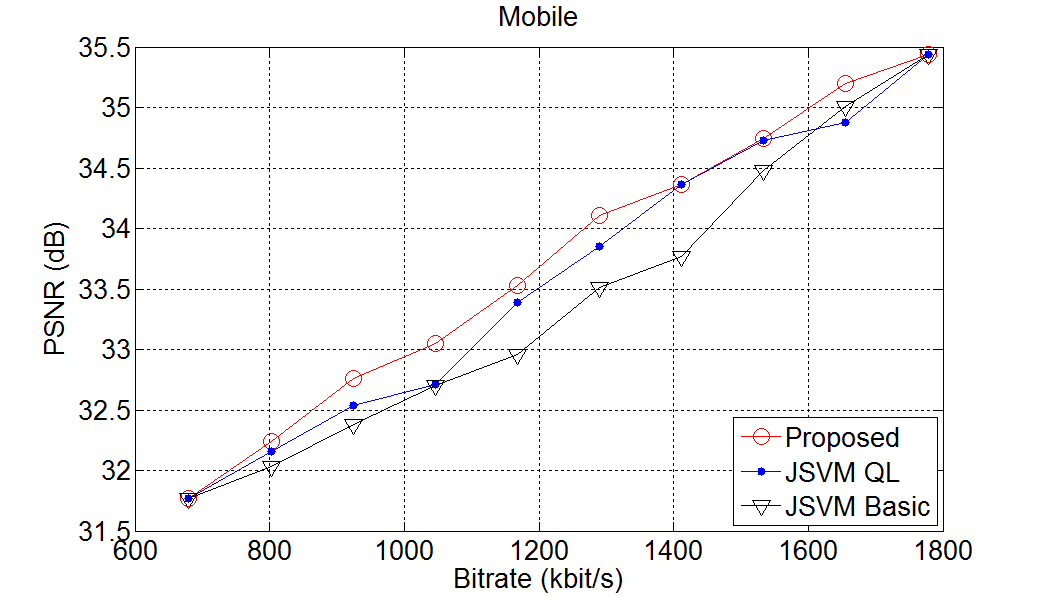
\includegraphics[width=0.5\textwidth]{figures/Mobile-noref.png}}
	\subfloat[Soccer]{
		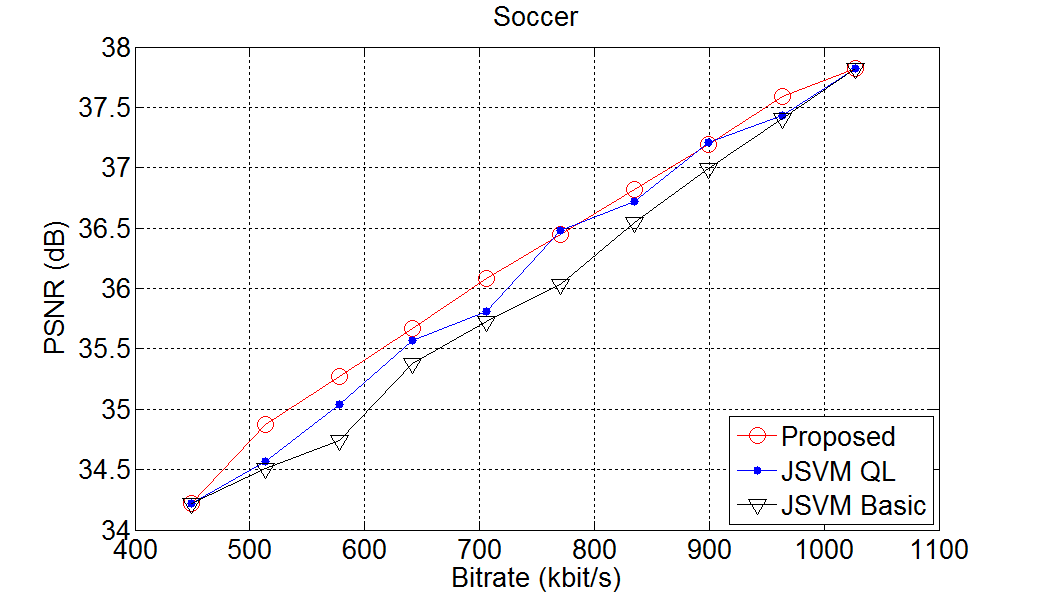
\includegraphics[width=0.5\textwidth]{figures/Soccer-noref.png}}
	\caption{无参考源时三种码流截取方案的性能比较}
	\label{fig:extraction-performance-noref}
\end{figure*}

对于无参考源的应用场景,我们也做了相应的实验。图\ref{fig:extraction-performance}展示了全部八个测试序列在无参考截取实验中的性能比较结果,直观地表明了本文所提方案取得了较好的率失真性能。表\ref{tab:extraction-gain}列出了对应的PSNR提升数据,同样可以看出本文所提出的方案的优越性。

\begin{table*}[t]
	\centering
	\caption{无参考源时本文提出的截取方案相比于JSVM的PSNR提升}
	\label{tab:extraction-gain-noref}
	\small
	\begin{minipage}{1.0\linewidth}
		\centering
		\begin{tabular}{c|c|*{3}{p{0.9cm}<{\centering}|}*{4}{p{1.1cm}<{\centering}|}p{0.9cm}<{\centering}}
			%% |l|l| to left justify each column entry
			%% |c|c| to center each column entry
			%% use of \rule[]{}{} below opens up each row
			\hline \hline
			\multicolumn{2}{c|}{序列名} &
			{\em Bus} & {\em City} & {\em Crew} & {\em Football} & {\em Foreman} & {\em Harbour} & {\em Mobile} & {\em Soccer} \\ \hline 
			\multirow{2}{*}{JSVM QL, $K$ = 32 \footnote{\label{footnote:JSVM_QL-noref} 与JSVM QL对比;优化窗口大小为32帧}}
			& Max\footnote{\label{footnote:max-noref} 所有码率限制下的最大提升}
			& 0.36 & 0.56 & 0.41 & 0.31 & 0.45 & 0.30 & 0.34 & 0.30 \\ \cline{2-10}
			& Ave\footnote{\label{footnote:ave-noref} 所有码率限制下的平均提升}
			& 0.14 & 0.22 & 0.13 & 0.12 & 0.17 & 0.11 & 0.14 & 0.11 \\ \hline
			\multirow{2}{*}{JSVM Basic, $K$ = 32}
			& Max & 0.48 & 0.97 & 0.54 & 0.25 & 0.47 & 0.38 & 0.60 & 0.53 \\ \cline{2-10}
			& Ave & 0.23 & 0.48 & 0.23 & 0.12 & 0.28 & 0.21 & 0.31 & 0.26 \\ \hline
		\end{tabular}
	\end{minipage}
\end{table*}

为了进一步证明本文提出的码流截取方案在无参考情况下的有效性,我们除了与JSVM对比,还做了进一步的对比实验。比较对象一方面选了Maani等人的方法\supercite{Maani2009},另一方面选了不进行本文\ref{subsec:noref}小节中的修改而直接采用公式(\ref{eq:R-D_impact_i})的方法。表\ref{tab:methods-compare}列出了三种不同的无参考截取方法相对于JSVM QL的平均PSNR提升。可以看出,Maani等人的方法在无参考情况下跟本文的方法性能相差无几,而在进行本文\ref{subsec:noref}小节中的修改之前,直接采用公式(\ref{eq:R-D_impact_i})则性能差了许多,甚至在有些序列上取得了比JSVM QL还差的结果。这进一步说明了\ref{subsec:noref}小节中修改的重要性。

\begin{table*}[t]
	\centering
	\caption{不同的无参考截取方法对比:相对于JSVM QL的平均PSNR提升}
	\label{tab:methods-compare}
	\small
	\begin{minipage}{1.0\linewidth}
		\centering
		\begin{tabular}{c|*{3}{p{0.9cm}<{\centering}|}*{4}{p{1.1cm}<{\centering}|}p{0.9cm}<{\centering}}
			\hline \hline
			序列名 & {\em Bus} & {\em City} & {\em Crew} & {\em Football} & {\em Foreman} & {\em Harbour} & {\em Mobile} & {\em Soccer} \\ \hline
			本文方法  & 0.14 & 0.22 & 0.13 & 0.12 & 0.17 & 0.11 & 0.14 & 0.11 \\ \cline{1-9}
			Maani等人的方法\supercite{Maani2009} & 0.13 & 0.22 & 0.13 & 0.11 & 0.16 & 0.02 & 0.08 & 0.12 \\ \cline{1-9}
			采用公式(\ref{eq:R-D_impact_i})方法 & 0.06 & 0.07 & 0.01 & 0.10 & 0.05 & 0.04 & -0.03 & -0.01 \\ \hline
		\end{tabular}
	\end{minipage}
\end{table*}

\section{本章小结}

本章介绍了一个采用线性误差模型的可伸缩视频码流截取方案。我们从H.264/AVC解码过程的线性性质推导出了质量可伸缩情况下的线性误差模型。该模型能使我们准确地估计丢弃任意数据包所带来的失真变化。基于此,我们设计了一个贪心算法来根据数据包的码率失真影响来为其赋优先级值,并按照这些优先级值来进行码流截取。实验表明,本文提出的线性误差模型对失真估计的误差率只有5\%,而采用该模型的码流截取相比于参考软件中的截取器有高达0.5dB的PSNR提升。本章的工作使得视频流媒体的数据源能够以很高的精度改变码率,为下一章要介绍的码率自适应提供了条件。